\section{Results}
\label{sec:results}

In this section, we evaluate our flagship DINOv3 7B model on a variety of computer vision tasks.
Throughout our experiments, unless otherwise specified, \emph{we keep DINOv3 frozen} and solely use its representations.
We demonstrate that with DINOv3, finetuning is not necessary to obtain strong performance.
This section is organized as follows. We first probe the quality of DINOv3's dense (\cref{sec:results-dense-features}) and global (\cref{sec:results-global-features}) image representations using lightweight evaluation protocols and compare it to the strongest available vision encoders. 
We show that DINOv3 learns exceptional dense features while offering robust and versatile global image representations.
Then, we consider DINOv3 as a basis for developing more complex computer vision systems (\cref{sec:results-system-level}).
We show with little effort on top of DINOv3, we are able to achieve results competitive with or exceeding the state of the art in tasks as diverse as object detection, semantic segmentation, 3D view estimation, or relative monocular depth estimation.

\subsection{DINOv3 provides Exceptional Dense Features}
\label{sec:results-dense-features}
We first investigate the raw quality of DINOv3's dense representations using a diverse set of lightweight evaluations.
In all cases, we utilize the frozen patch features of the last layer, and evaluate them using 
(1) qualitative visualizations (\cref{sec:results-qualitative}), 
(2) dense linear probing (\cref{sec:results-dense-linear-probing}: segmentation, depth estimation),
(3) non-parametric approaches (\cref{sec:results-correspondence-estimation}: 3D correspondence estimation, \cref{sec:results-object-discovery}: object discovery, \cref{sec:results-tracking}: tracking), 
and (4) lightweight attentive probing (\cref{sec:results-video-classification}: video classification).

\paragraph{Baselines}
We compare the dense features of DINOv3 with those of the strongest publicly available image encoders, both weakly- and self-supervised ones. 
We consider the weakly-supervised encoders Perception Encoder (PE) Core~\citep{bolya2025perception} and SigLIP 2~\citep{tschannen2025siglip}, which use CLIP-style image-text contrastive learning.
We also compare to the strongest self-supervised methods: DINOv3's predecessor DINOv2~\citep{oquab2024dinov2} with registers~\citep{darcet2024vision}, Web-DINO~\citep{fan2025scaling}, a recent scaling effort of DINO, and Franca~\citep{venkataramanan2025franca}, the best open-data SSL model.   %
Finally, we compare to the agglomerative models AM-RADIOv2.5~\citep{heinrich2025radiov25}, distilled from DINOv2, CLIP~\citep{radford2021learning}, DFN~\citep{fang2024data}, and Segment Anything (SAM)~\citep{kirillov2023segment}, and to PEspatial, distilling SAM 2~\citep{ravi2025sam} into PEcore.
For each baseline, we report the performance of the strongest model available and specify the architecture in the tables.

\subsubsection{Qualitative Analysis}
\label{sec:results-qualitative}
We start by analyzing DINOv3's dense feature maps qualitatively.
To this end, we project the dense feature space into 3 dimensions using principal component analysis (PCA), and map the resulting 3D space into RGB.
Because of the sign ambiguity in PCA (eight variants) and the arbitrary mapping between principal components and colors (six variants), we explore all combinations and report the visually most compelling one.
The resulting visualization is shown in \cref{fig:results-pca}.
Compared to other vision backbones, it can be seen that the features of DINOv3 are sharper, containing much less noise, and showing superior semantical coherence.

\begin{figure}[t]
    \centering
    \begin{subfigure}{0.195\textwidth}
        \centering
        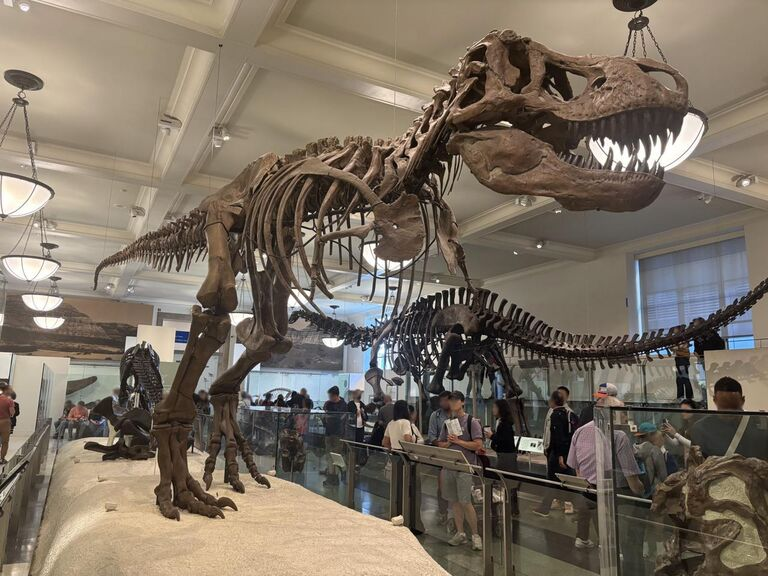
\includegraphics[width=\linewidth]{images/pca_comparison/img_3.lr.jpg}
    \end{subfigure}\hfill
    \begin{subfigure}{0.195\textwidth}
        \centering
        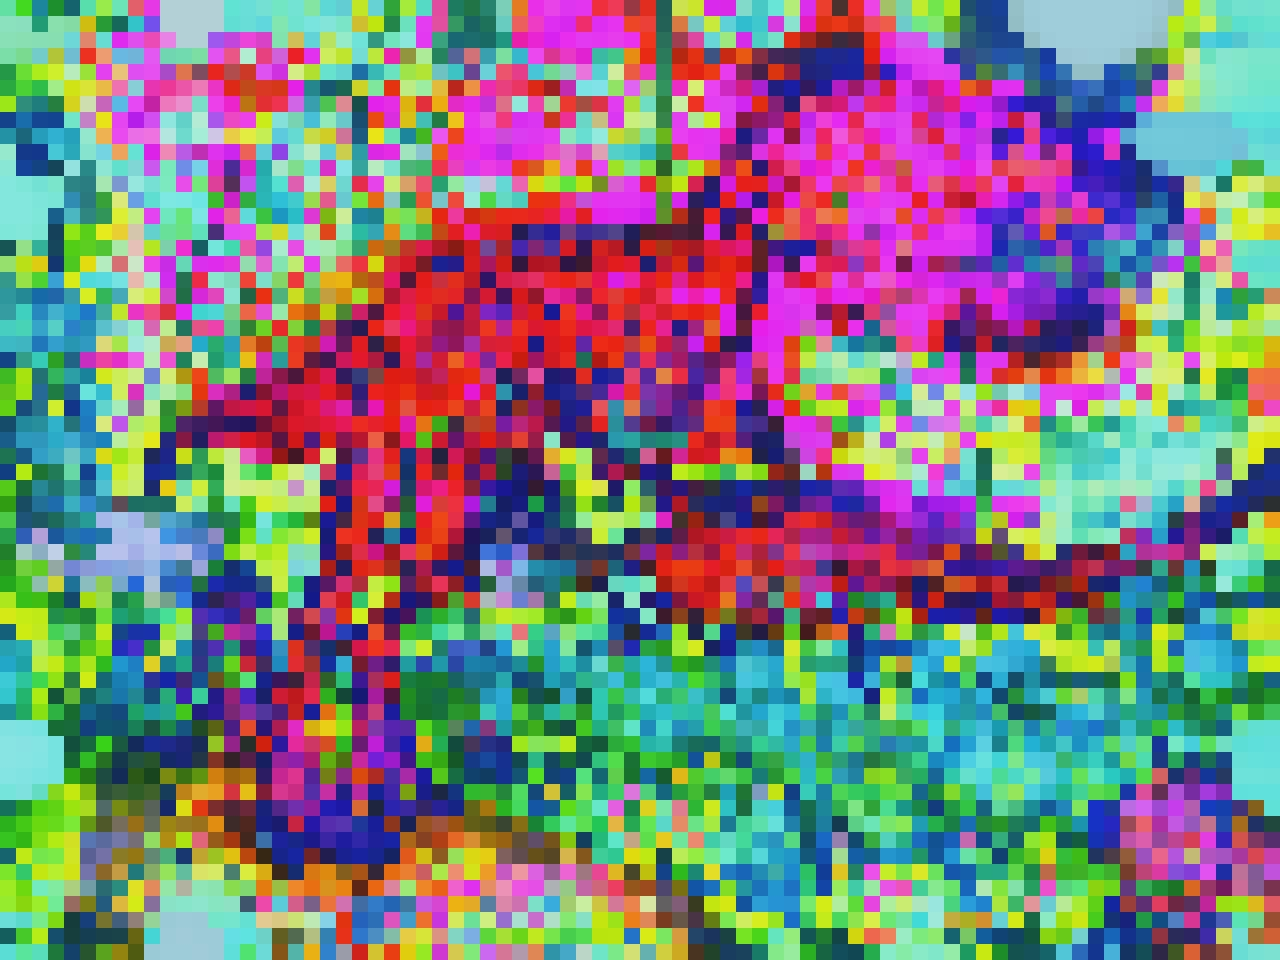
\includegraphics[width=\linewidth]{images/pca_comparison/siglip2/3_m0p1p2.jpg}
    \end{subfigure}\hfill
    \begin{subfigure}{0.195\textwidth}
        \centering
        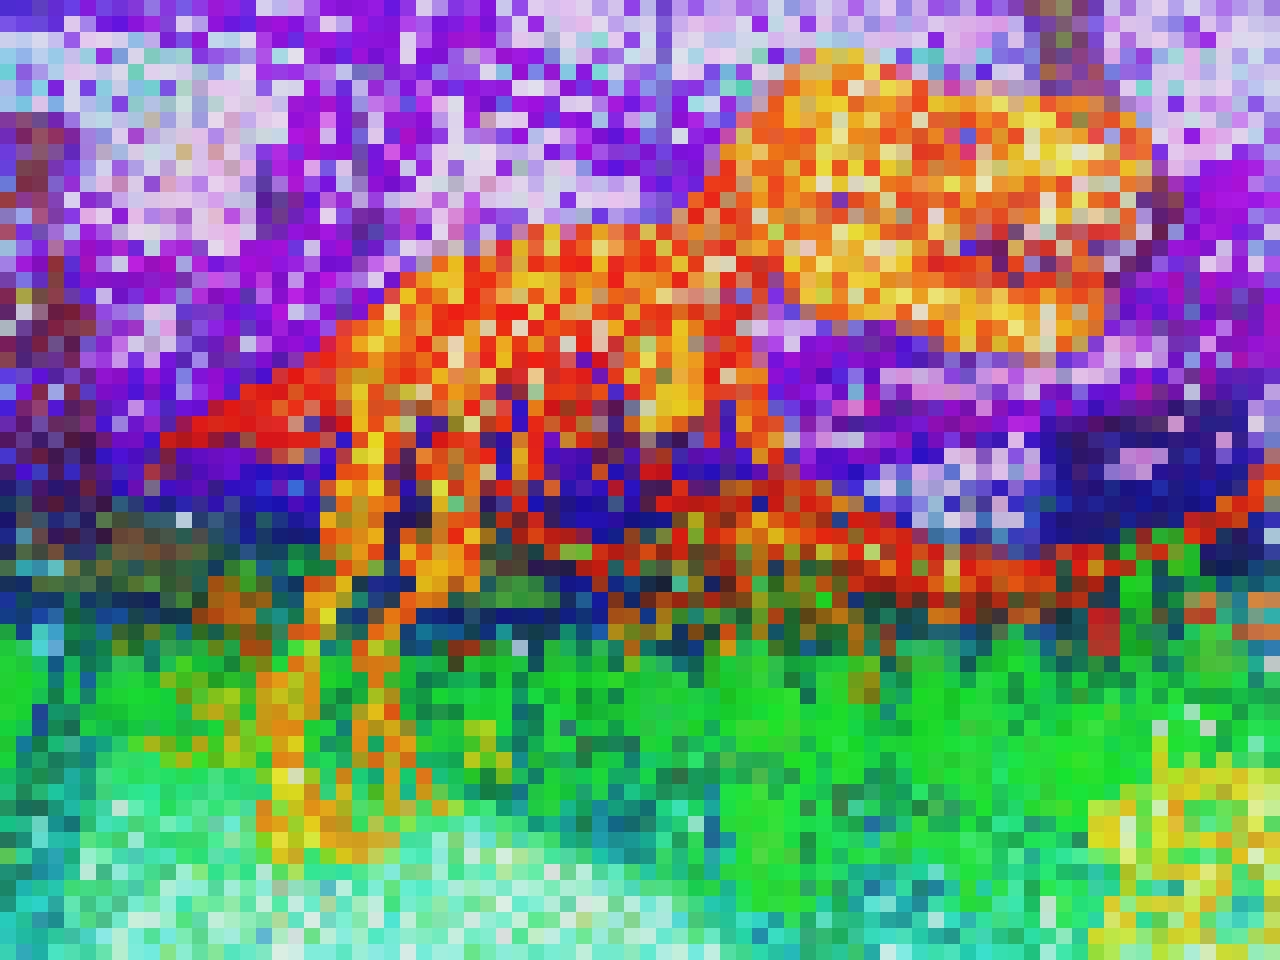
\includegraphics[width=\linewidth]{images/pca_comparison/pe_spatial/3_p1p2p0.jpg}
    \end{subfigure}\hfill
    \begin{subfigure}{0.195\textwidth}
        \centering
        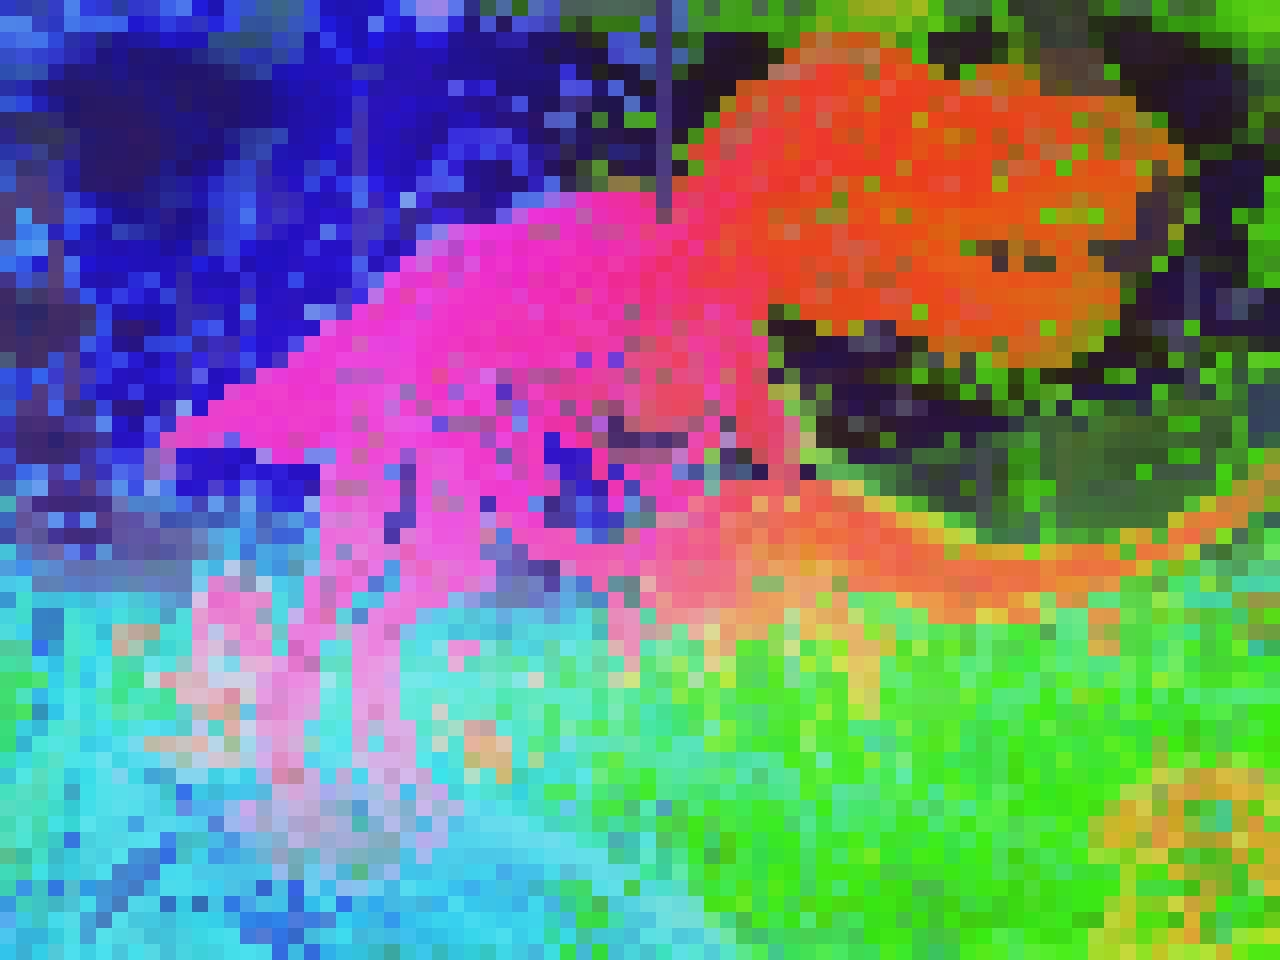
\includegraphics[width=\linewidth]{images/pca_comparison/dinov2/3_m0p1m2.jpg}
    \end{subfigure}\hfill
    \begin{subfigure}{0.195\textwidth}
        \centering
        
\includegraphics[width=\linewidth]{images/pca_comparison/dinov3/3_m0p1m2.jpg}
    \end{subfigure}\vspace{0.25em}
    \begin{subfigure}{0.195\textwidth}
        \centering
        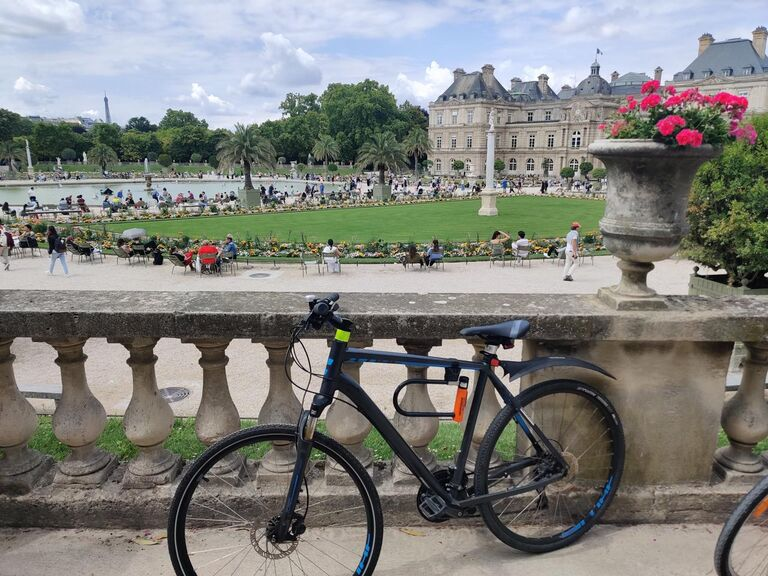
\includegraphics[width=\linewidth]{images/pca_comparison/img_2.lr.jpg}
    \end{subfigure}\hfill
    \begin{subfigure}{0.195\textwidth}
        \centering
        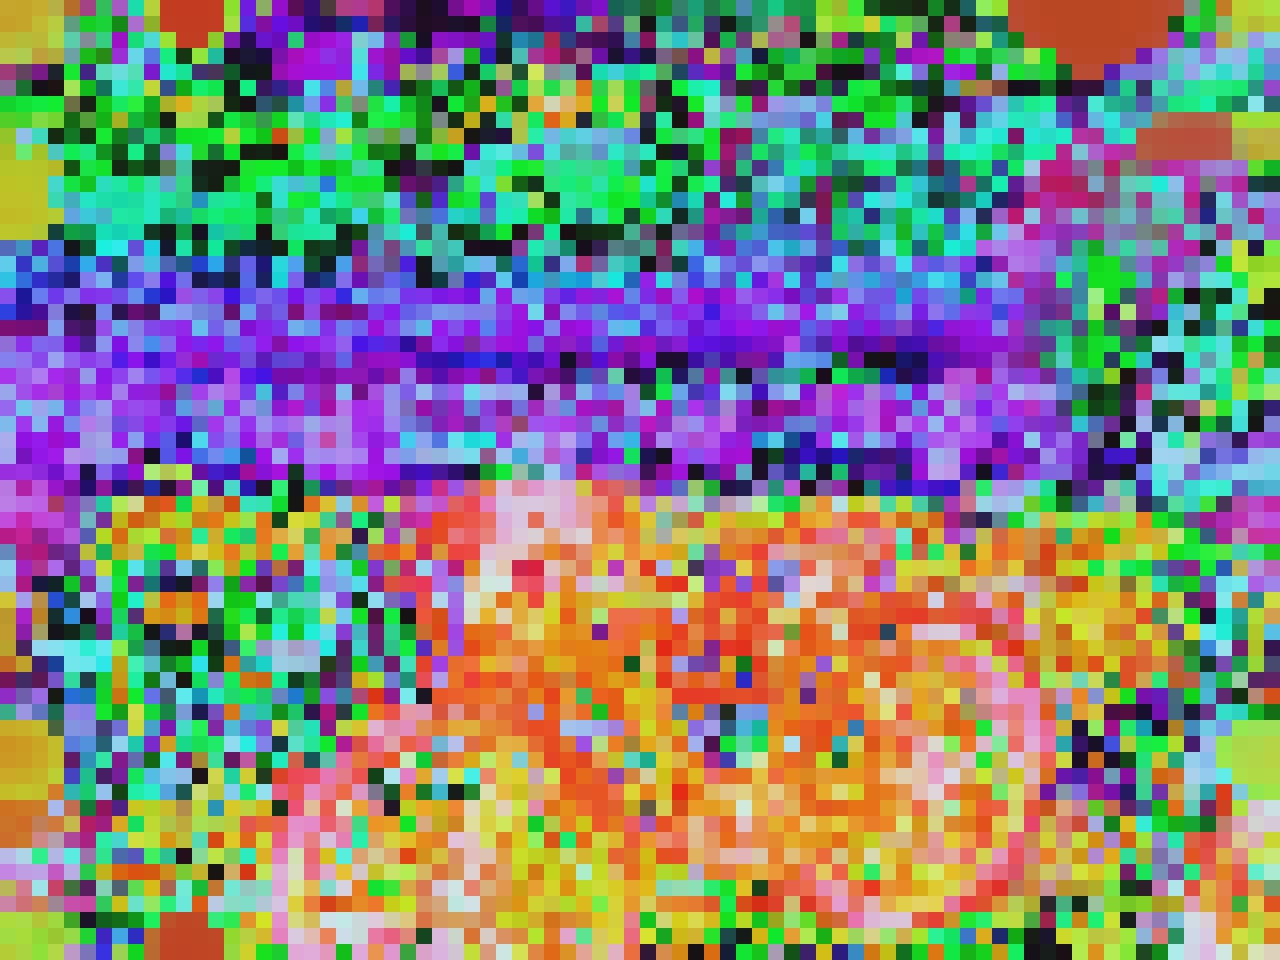
\includegraphics[width=\linewidth]{images/pca_comparison/siglip2/2_m0m2p1.jpg}
    \end{subfigure}\hfill
    \begin{subfigure}{0.195\textwidth}
        \centering
        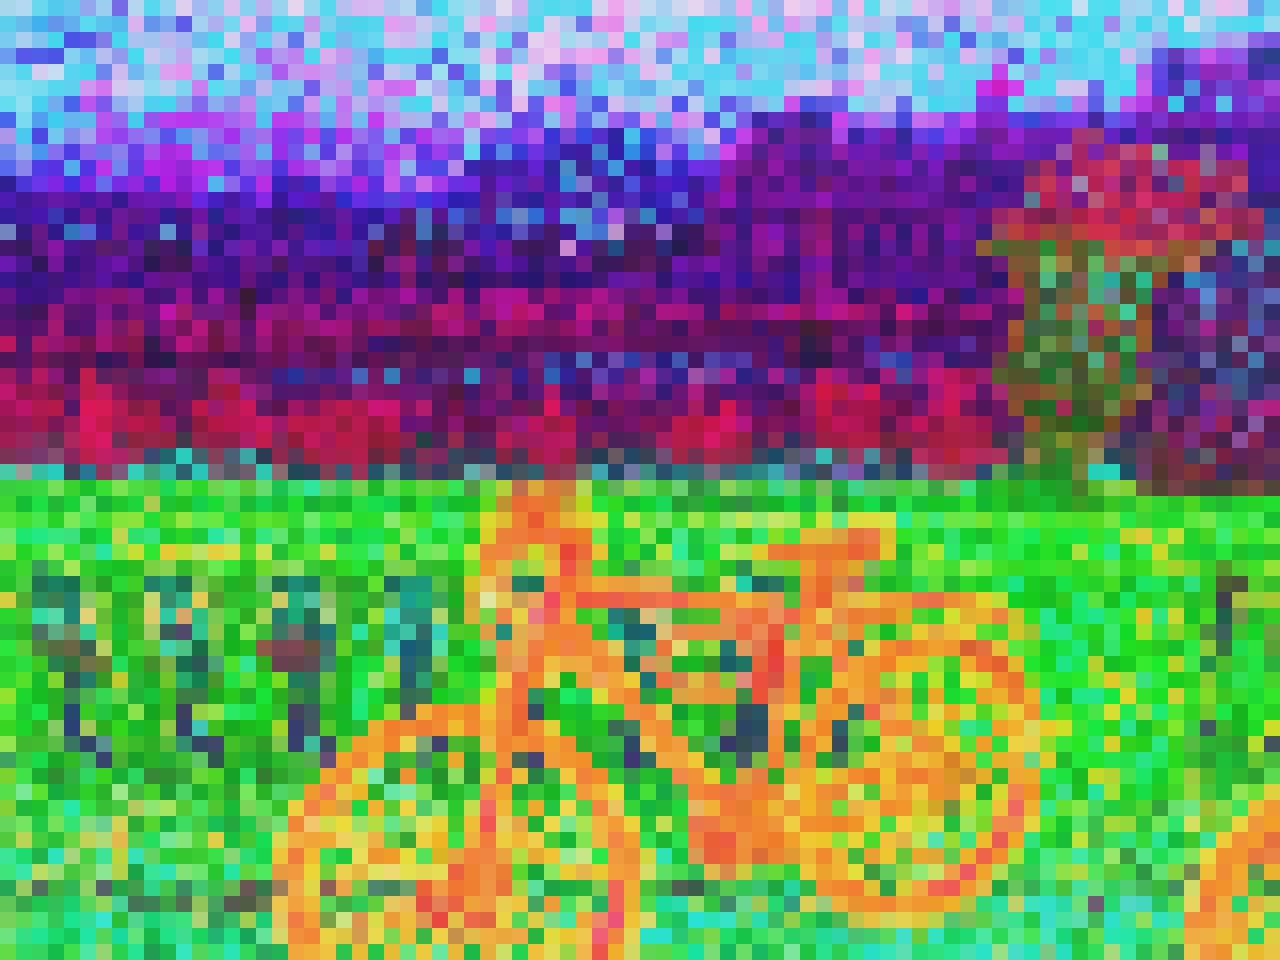
\includegraphics[width=\linewidth]{images/pca_comparison/pe_spatial/2_m2p1p0.jpg}
    \end{subfigure}\hfill
    \begin{subfigure}{0.195\textwidth}
        \centering
        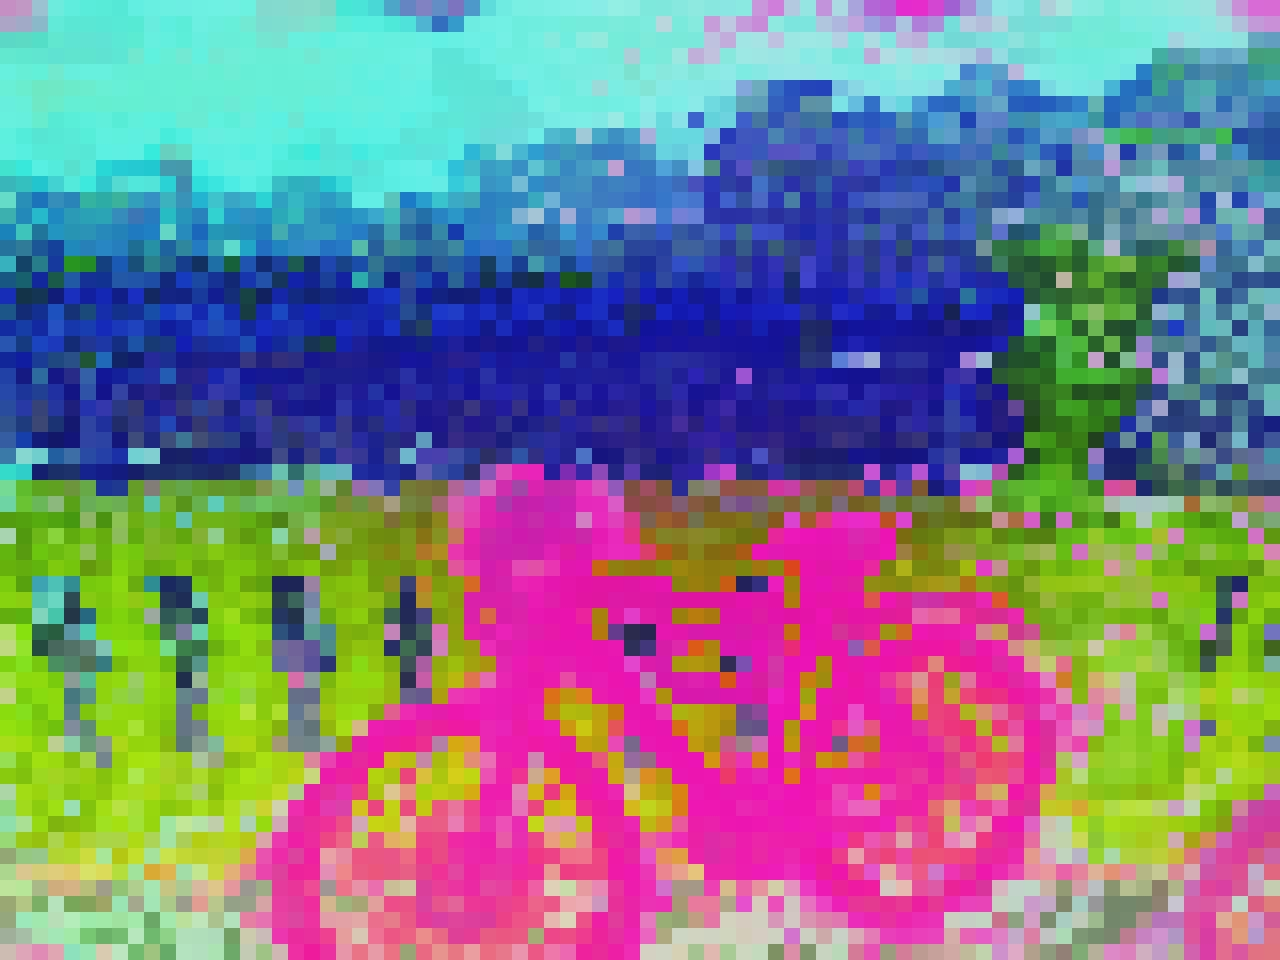
\includegraphics[width=\linewidth]{images/pca_comparison/dinov2/2_m0p2p1.jpg}
    \end{subfigure}\hfill
    \begin{subfigure}{0.195\textwidth}
        \centering
        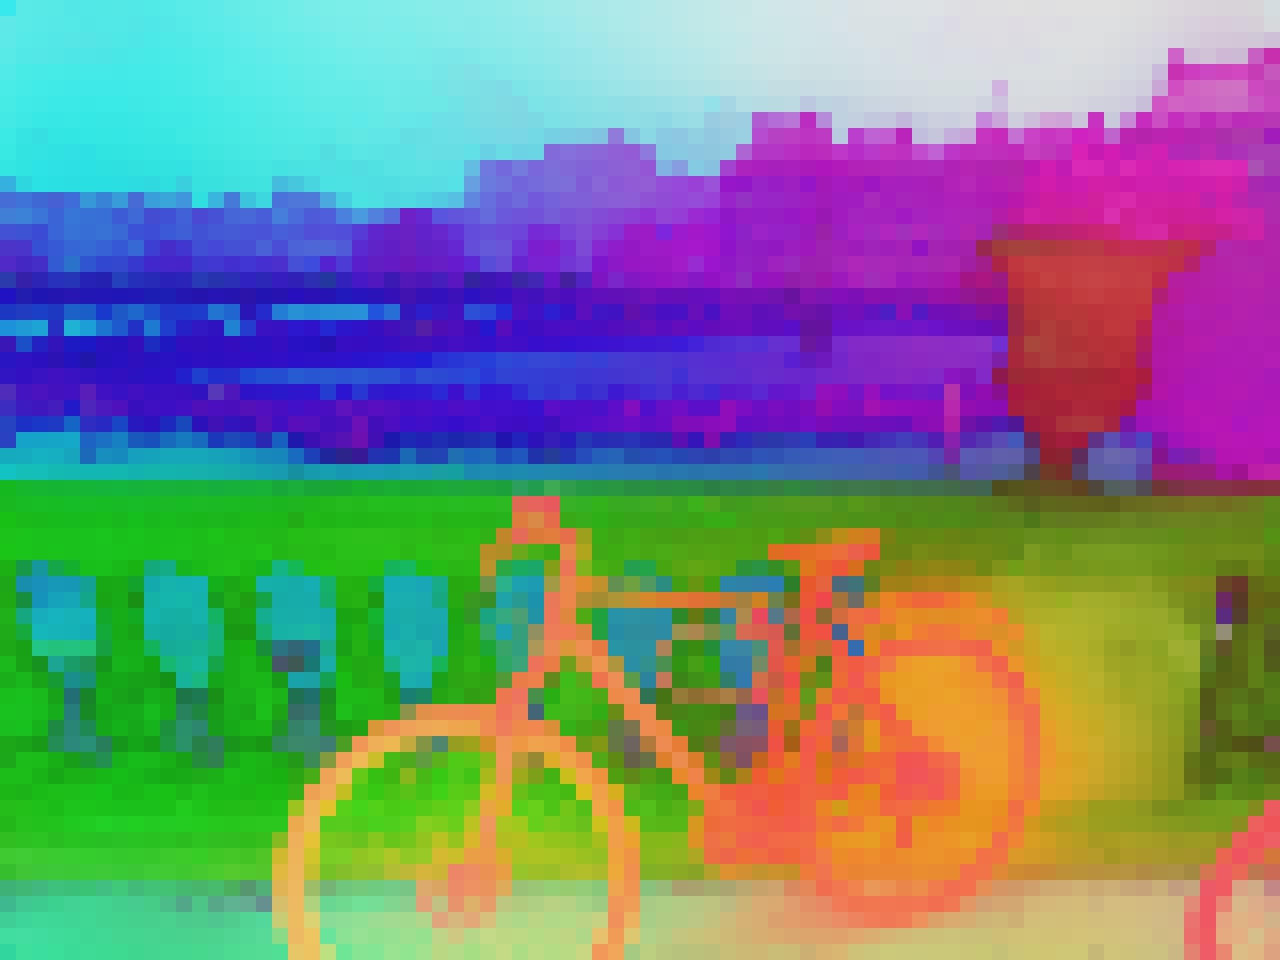
\includegraphics[width=\linewidth]{images/pca_comparison/dinov3/2_p2m1m0.jpg}
    \end{subfigure}\vspace{0.25em}
    \begin{subfigure}{0.195\textwidth}
        \centering
        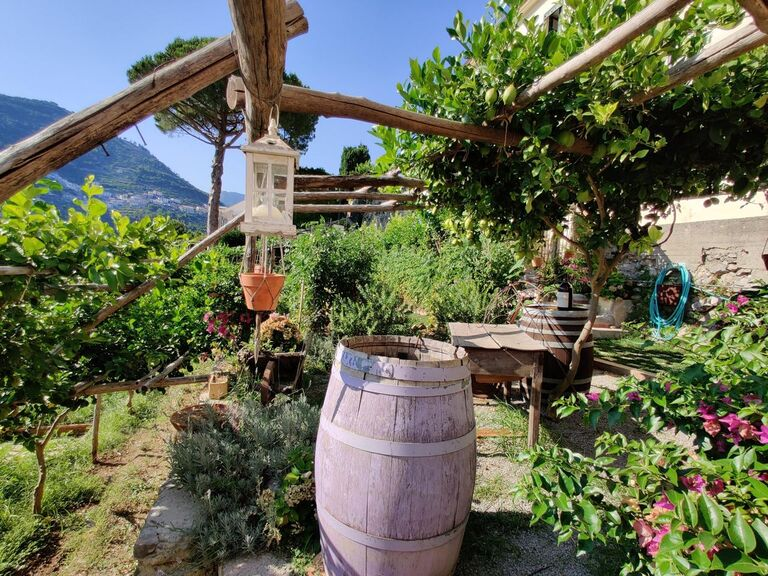
\includegraphics[width=\linewidth]{images/pca_comparison/img_1.lr.jpg}
    \end{subfigure}\hfill
    \begin{subfigure}{0.195\textwidth}
        \centering
        
\includegraphics[width=\linewidth]{images/pca_comparison/siglip2/1_m1m2p0.jpg}
    \end{subfigure}\hfill
    \begin{subfigure}{0.195\textwidth}
        \centering
        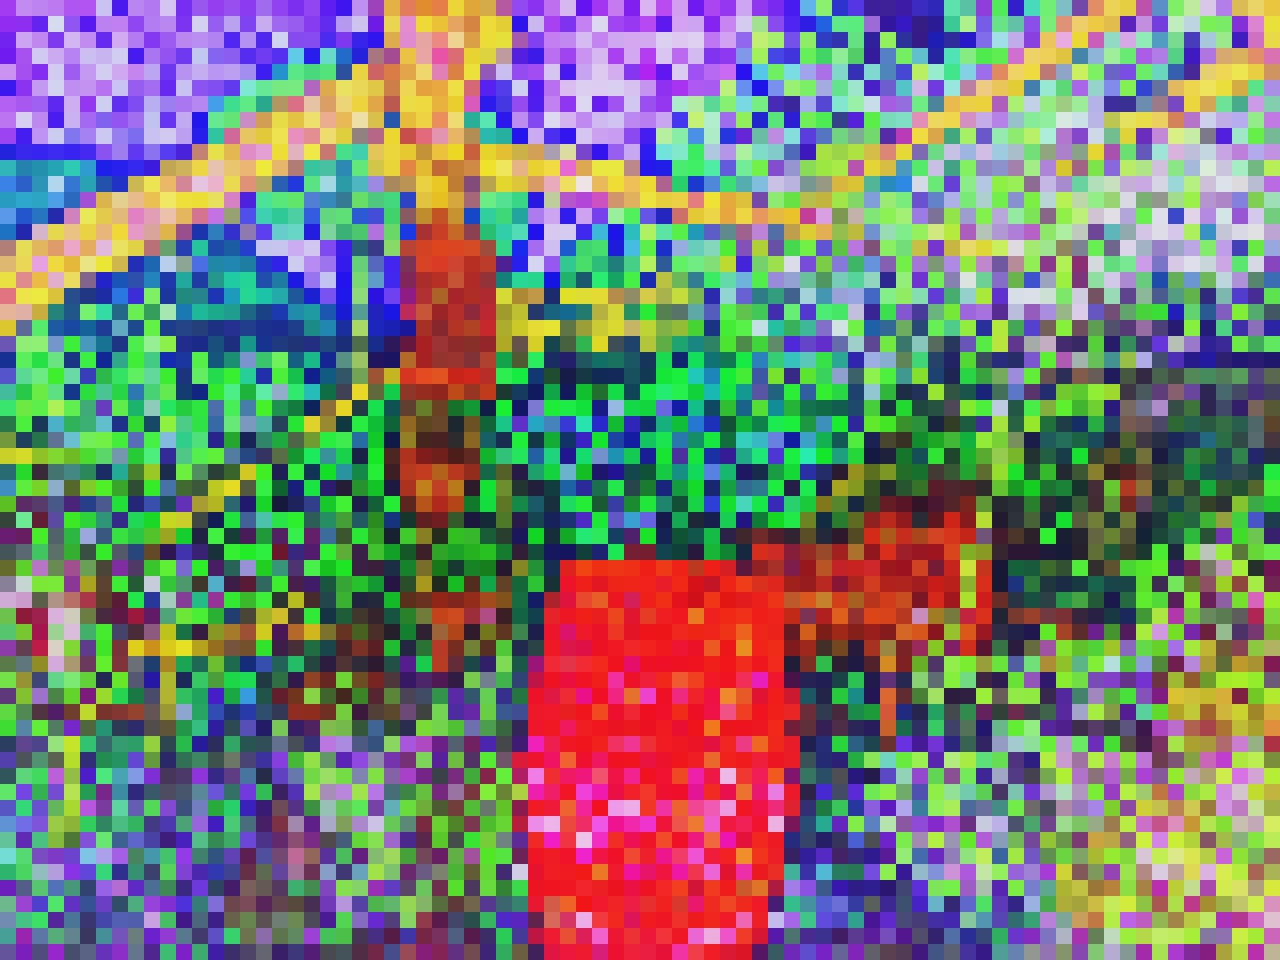
\includegraphics[width=\linewidth]{images/pca_comparison/pe_spatial/1_m1m2p0.jpg}
    \end{subfigure}\hfill
    \begin{subfigure}{0.195\textwidth}
        \centering
        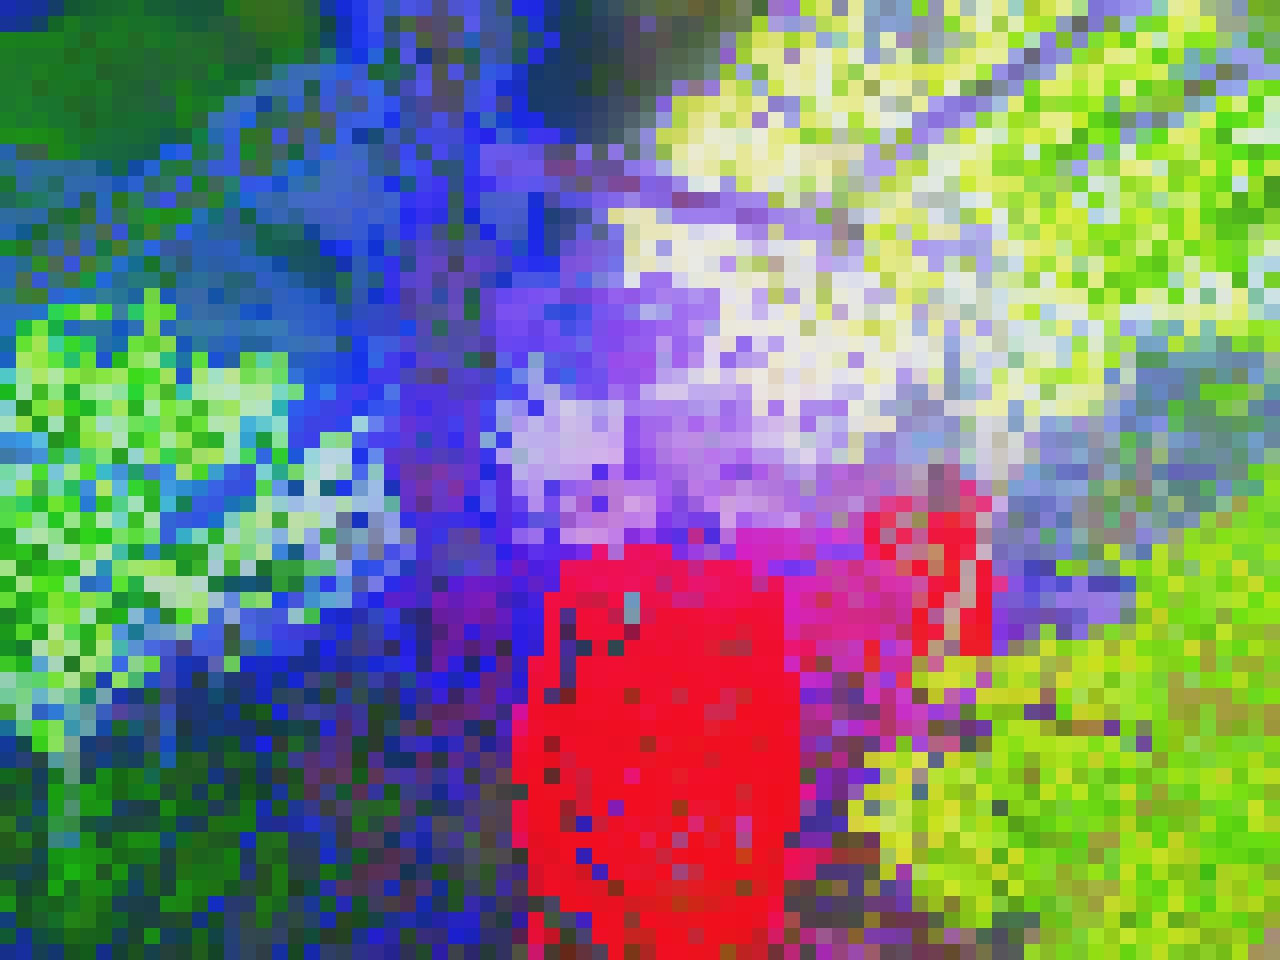
\includegraphics[width=\linewidth]{images/pca_comparison/dinov2/1_p1p0m2.jpg}
    \end{subfigure}\hfill
    \begin{subfigure}{0.195\textwidth}
        \centering
        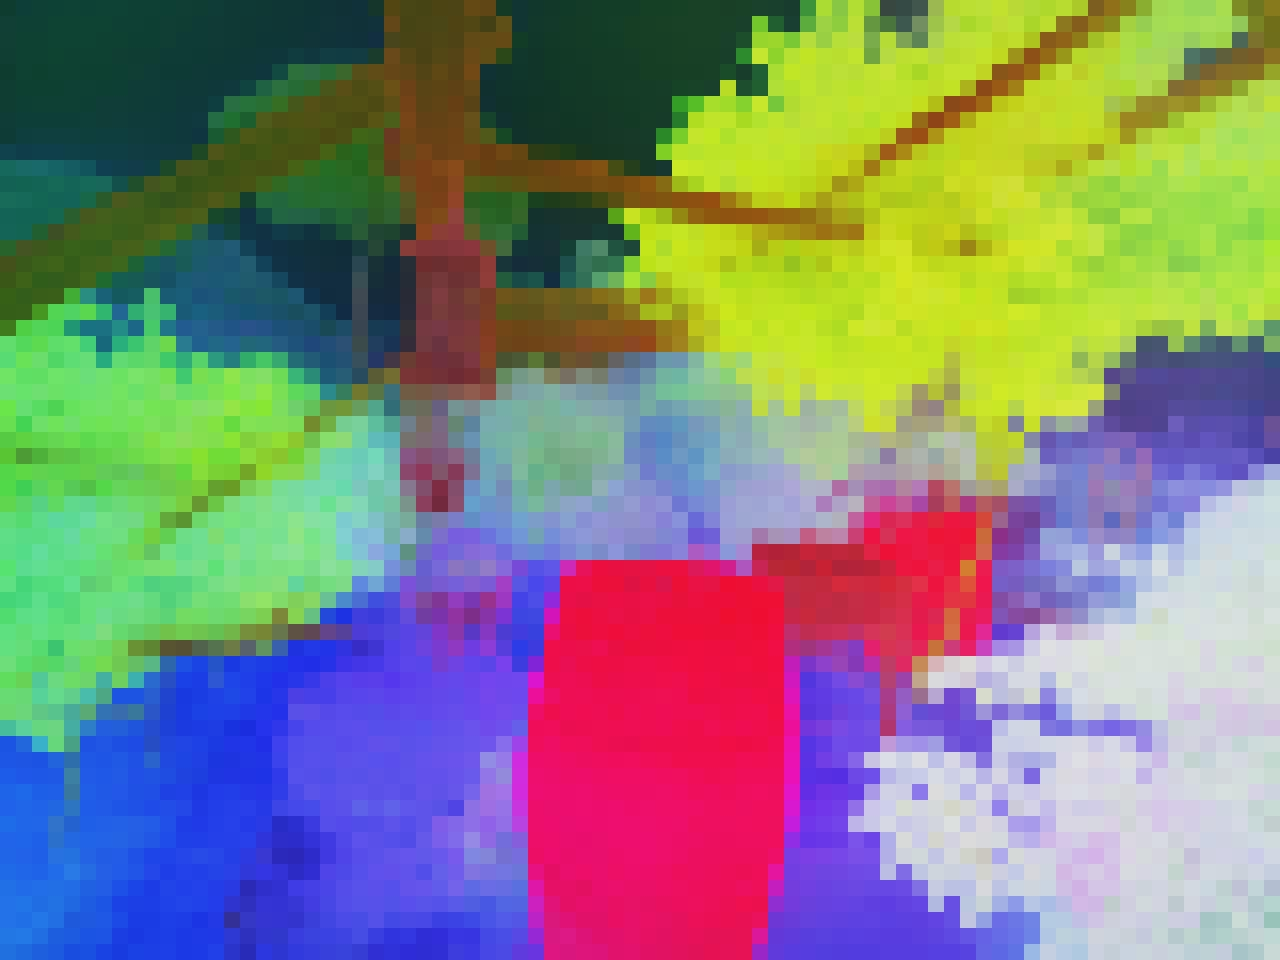
\includegraphics[width=\linewidth]{images/pca_comparison/dinov3/1_m1p0p2.jpg}
    \end{subfigure}\vspace{0.25em}
    \begin{subfigure}{0.195\textwidth}
        \centering
        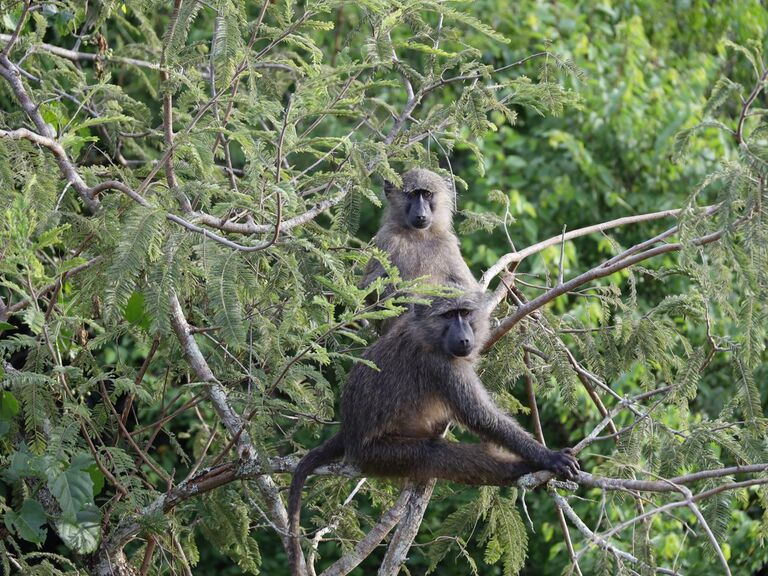
\includegraphics[width=\linewidth]{images/pca_comparison/img_4.lr.jpg}
    \end{subfigure}\hfill
    \begin{subfigure}{0.195\textwidth}
        \centering
        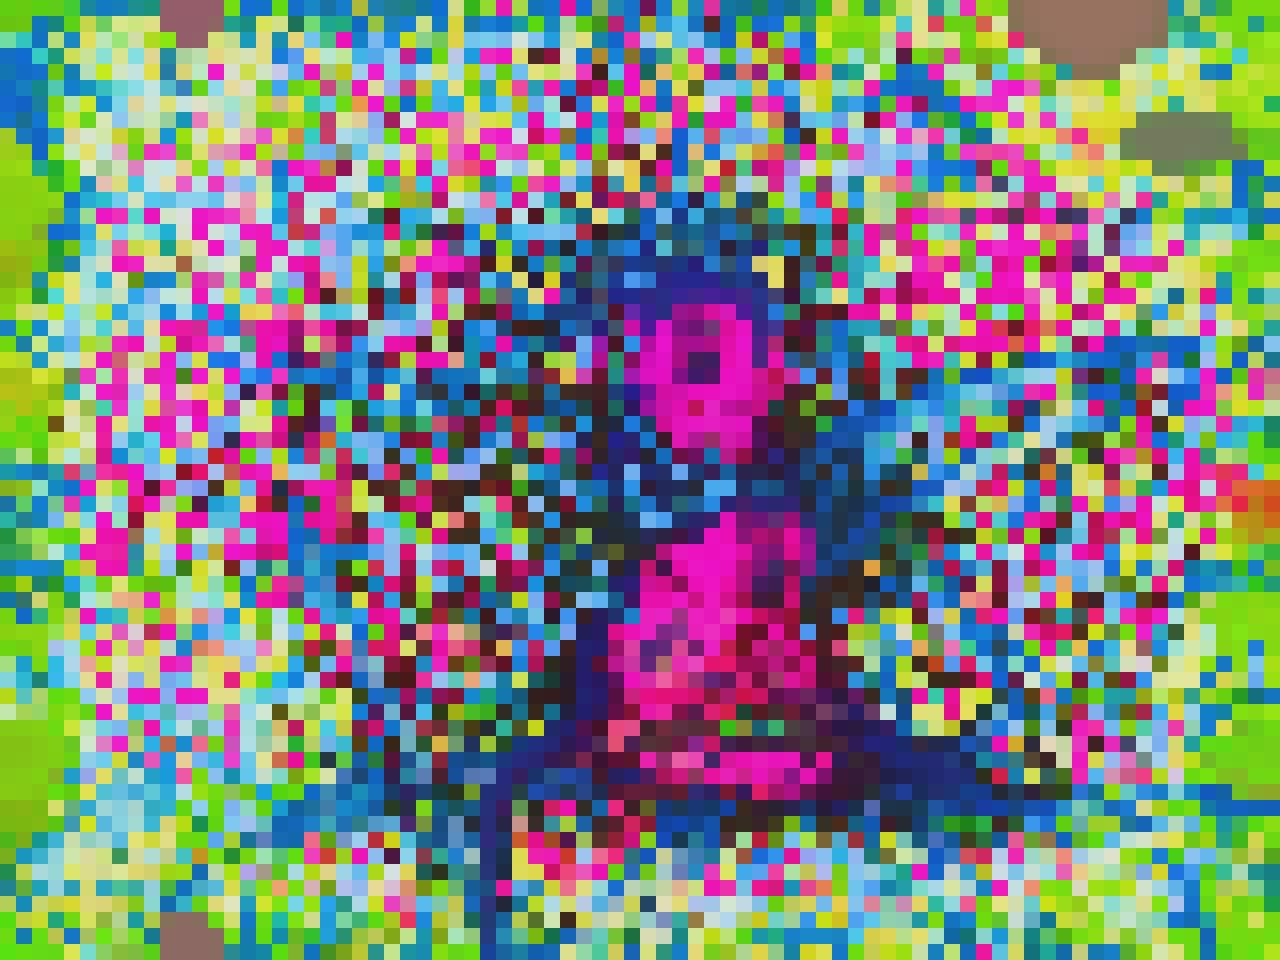
\includegraphics[width=\linewidth]{images/pca_comparison/siglip2/4_m0m1p2.jpg}
    \end{subfigure}\hfill
    \begin{subfigure}{0.195\textwidth}
        \centering
        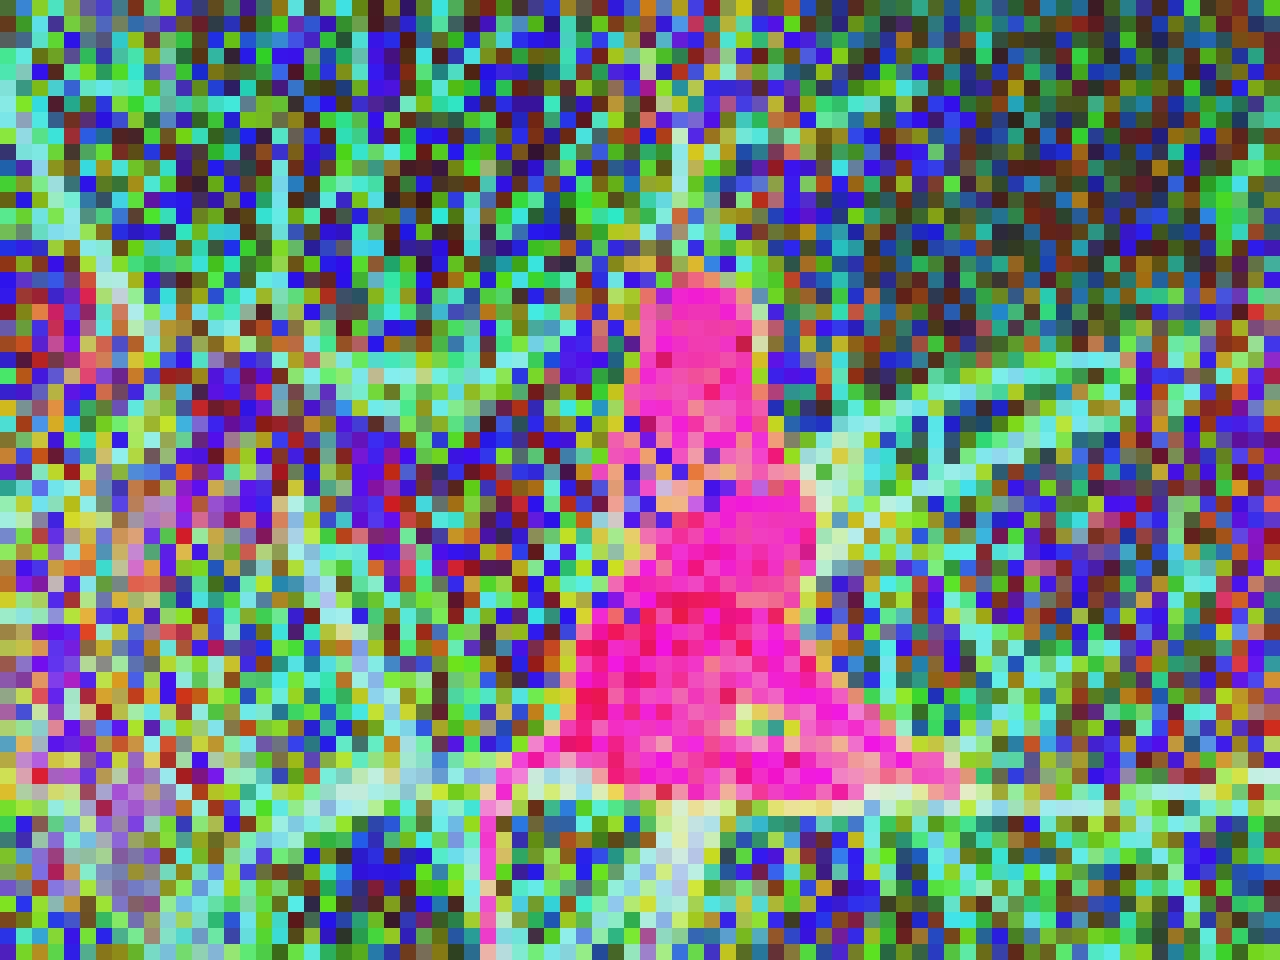
\includegraphics[width=\linewidth]{images/pca_comparison/pe_spatial/4_m0p2m1.jpg}
    \end{subfigure}\hfill
    \begin{subfigure}{0.195\textwidth}
        \centering
        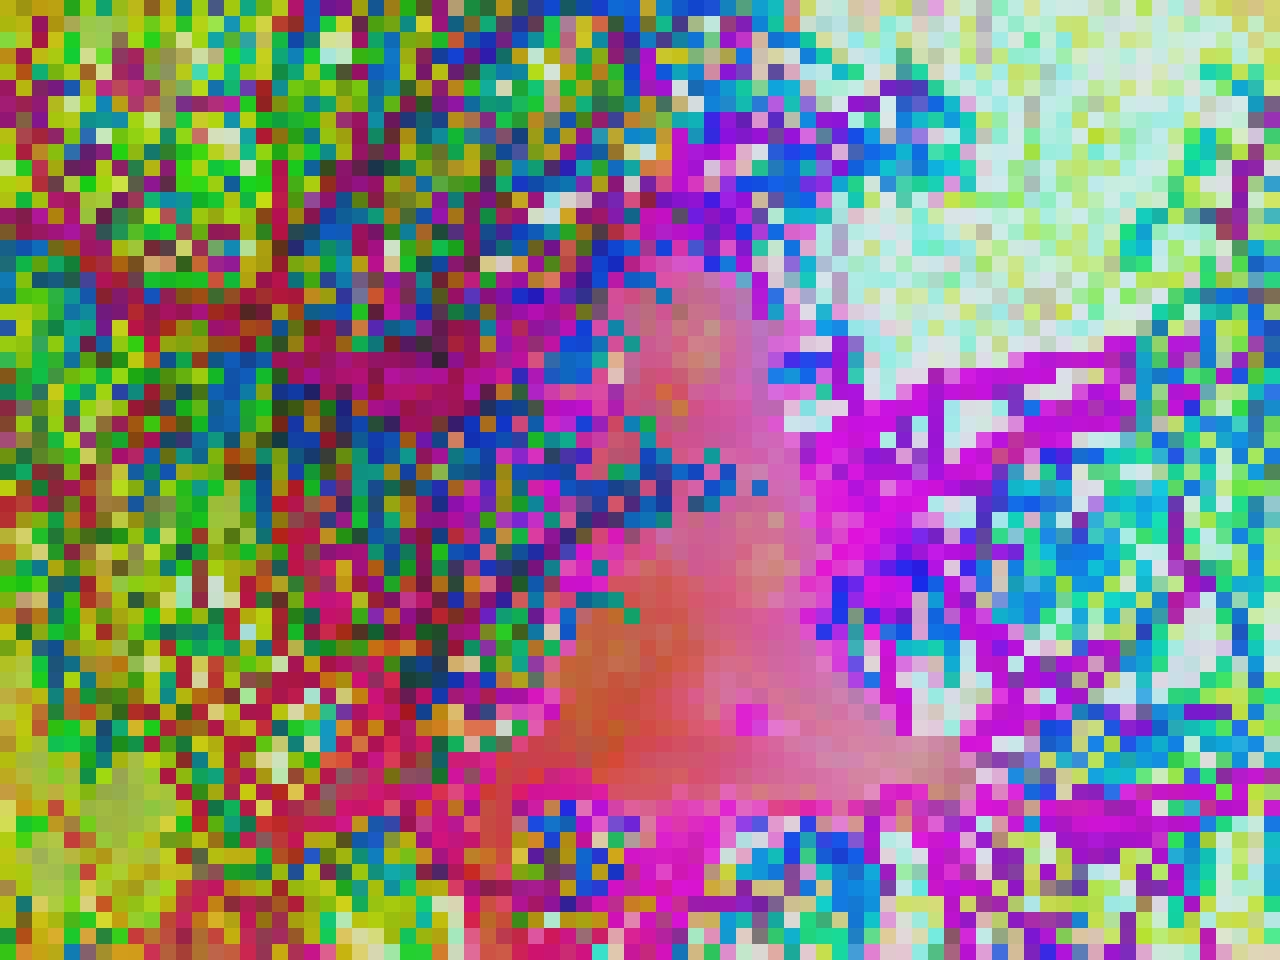
\includegraphics[width=\linewidth]{images/pca_comparison/dinov2/4_p0p1p2.jpg}
    \end{subfigure}\hfill
    \begin{subfigure}{0.195\textwidth}
        \centering
        
\includegraphics[width=\linewidth]{images/pca_comparison/dinov3/4_p0p1p2.jpg}
    \end{subfigure}\vspace{0.25em}
    \begin{subfigure}{0.195\textwidth}
        \centering
        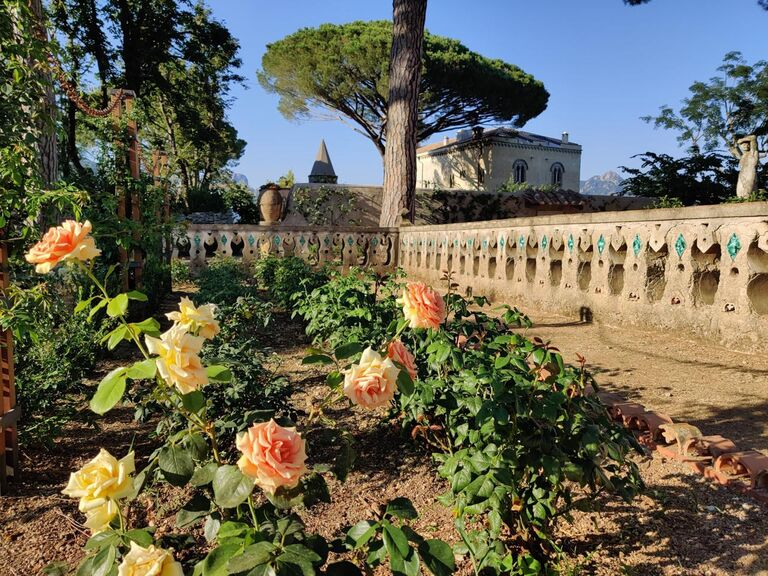
\includegraphics[width=\linewidth]{images/pca_comparison/img_0.lr.jpg}
    \end{subfigure}\hfill
    \begin{subfigure}{0.195\textwidth}
        \centering
        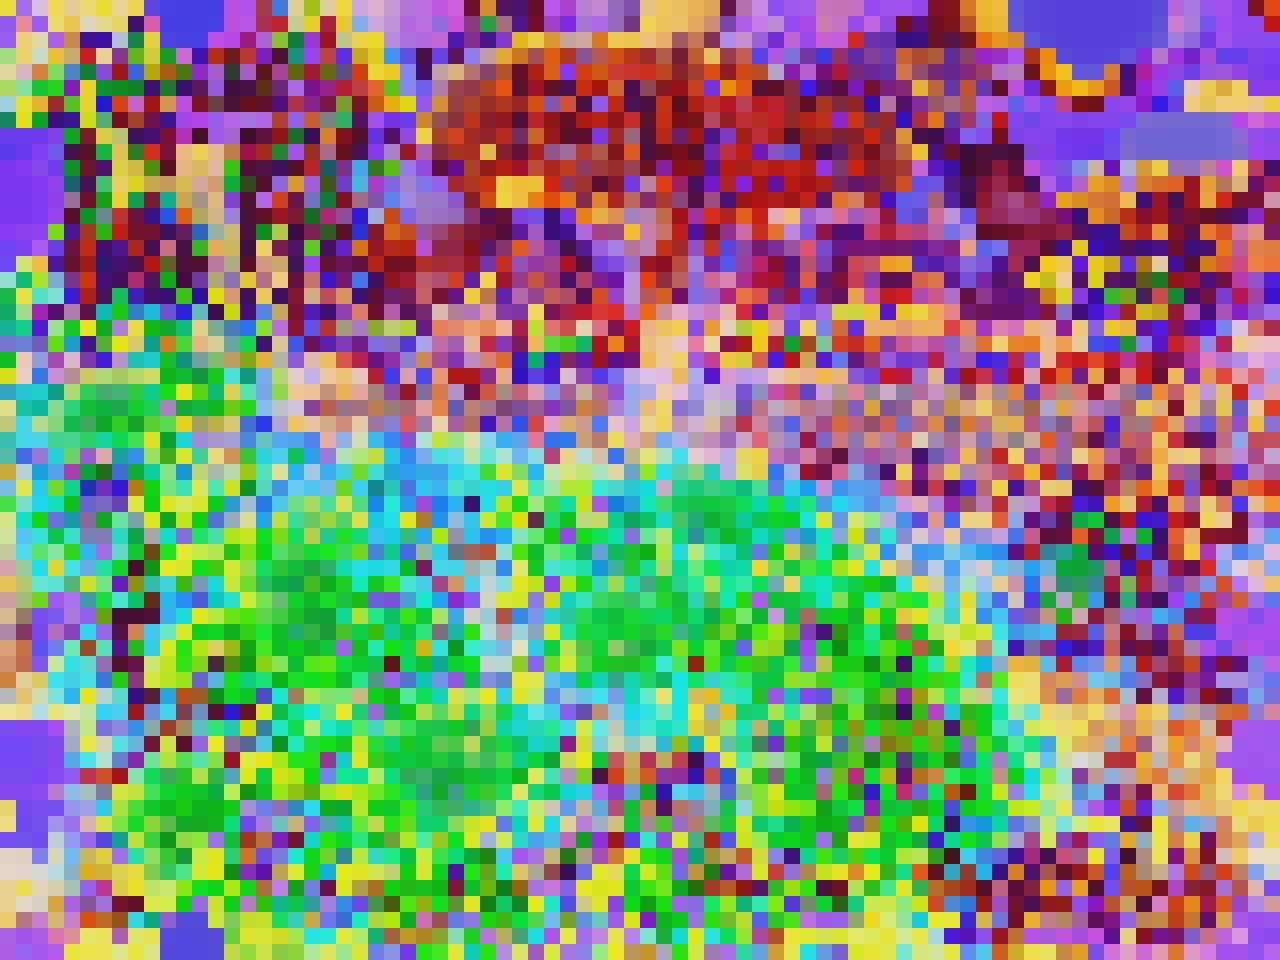
\includegraphics[width=\linewidth]{images/pca_comparison/siglip2/0_p2m0m1.jpg}
    \end{subfigure}\hfill
    \begin{subfigure}{0.195\textwidth}
        \centering
        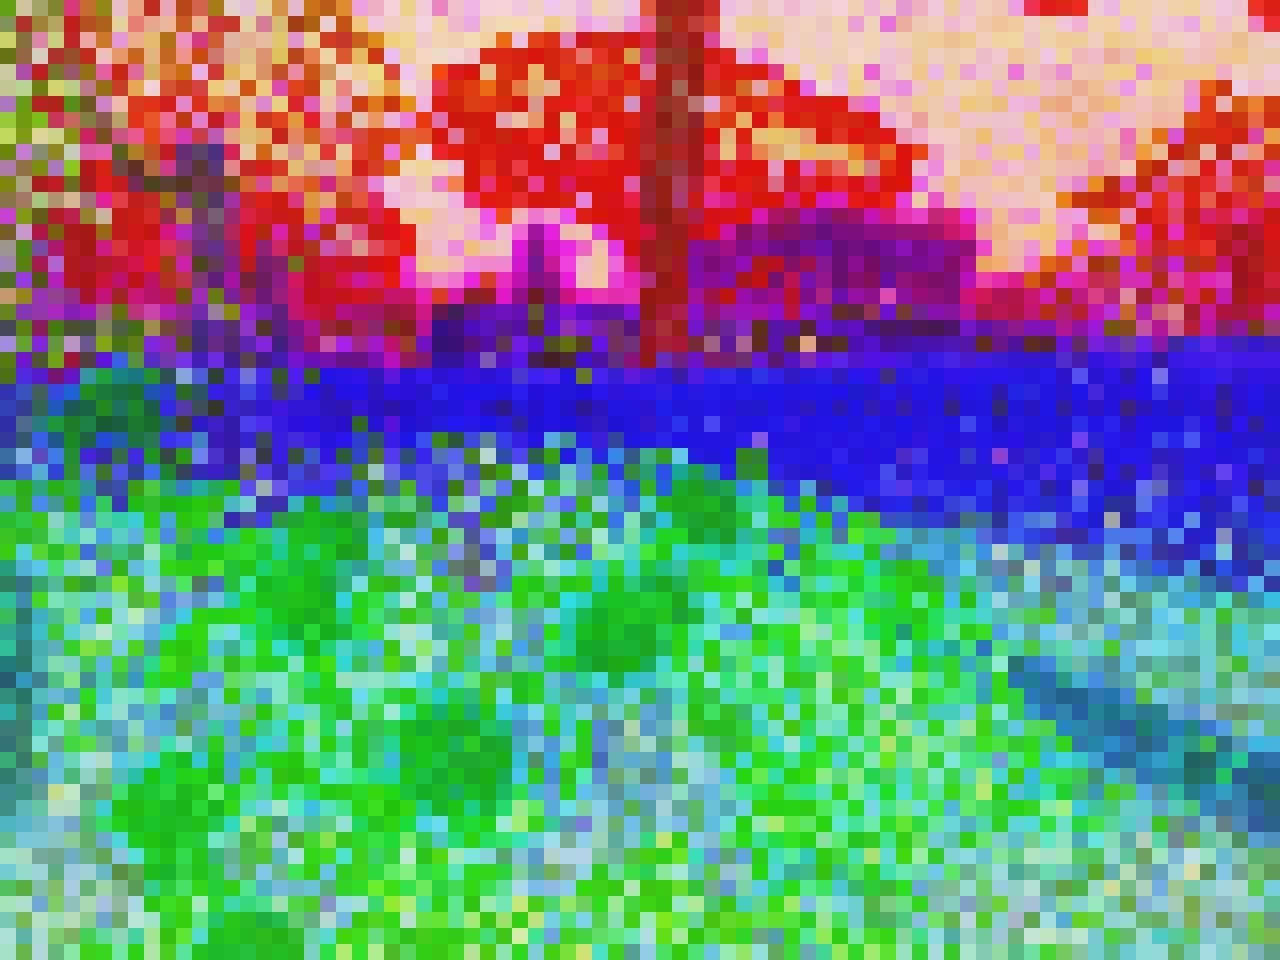
\includegraphics[width=\linewidth]{images/pca_comparison/pe_spatial/0_p0p1p2.jpg}
    \end{subfigure}\hfill
    \begin{subfigure}{0.195\textwidth}
        \centering
        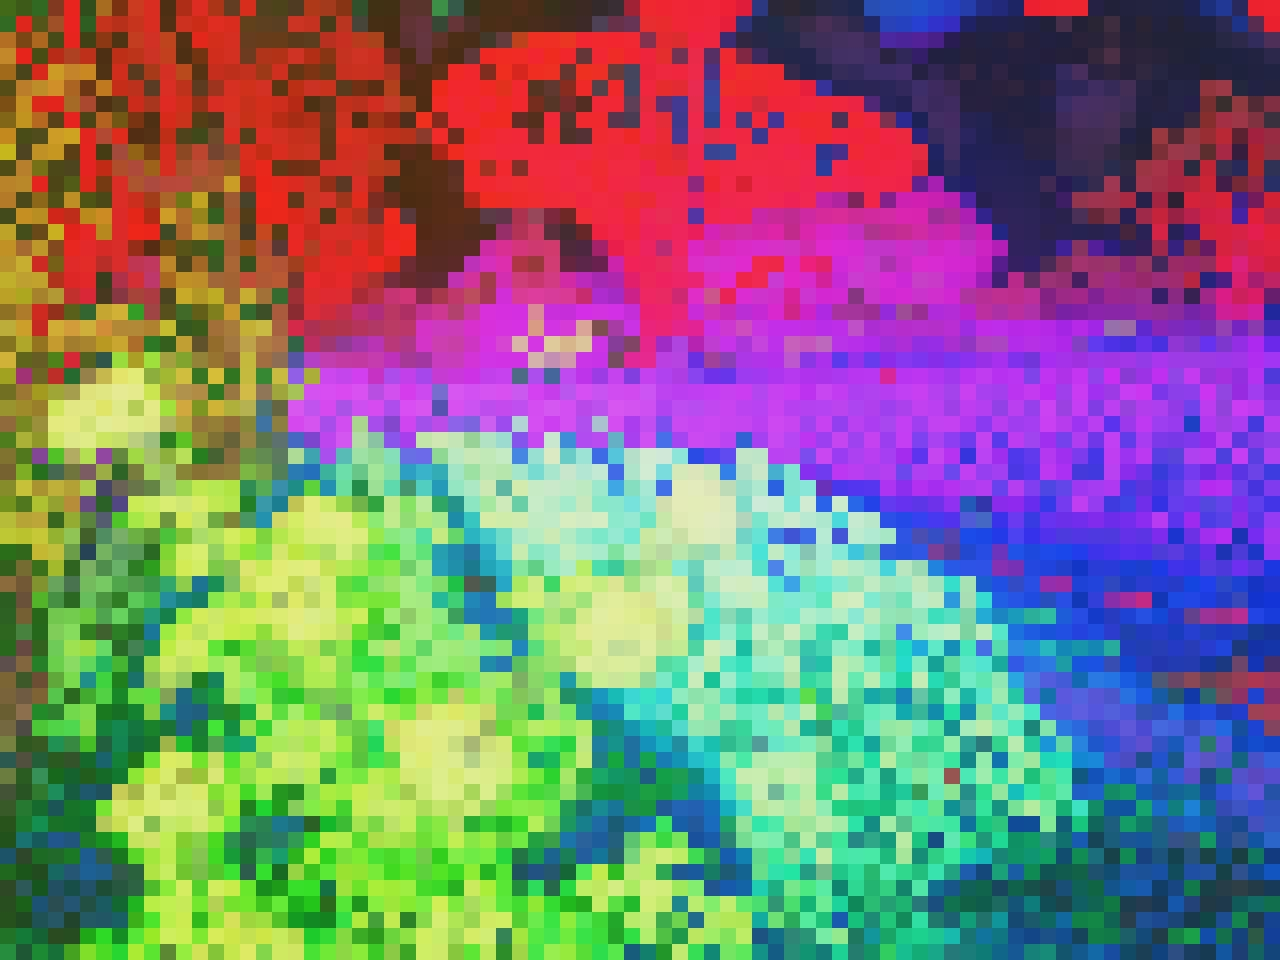
\includegraphics[width=\linewidth]{images/pca_comparison/dinov2/0_m2m0p1.jpg}
    \end{subfigure}\hfill
    \begin{subfigure}{0.195\textwidth}
        \centering
        
\includegraphics[width=\linewidth]{images/pca_comparison/dinov3/0_m2m0p1.jpg}
    \end{subfigure}\vspace{0.25em}
    \begin{subfigure}{0.195\textwidth}
        \centering
        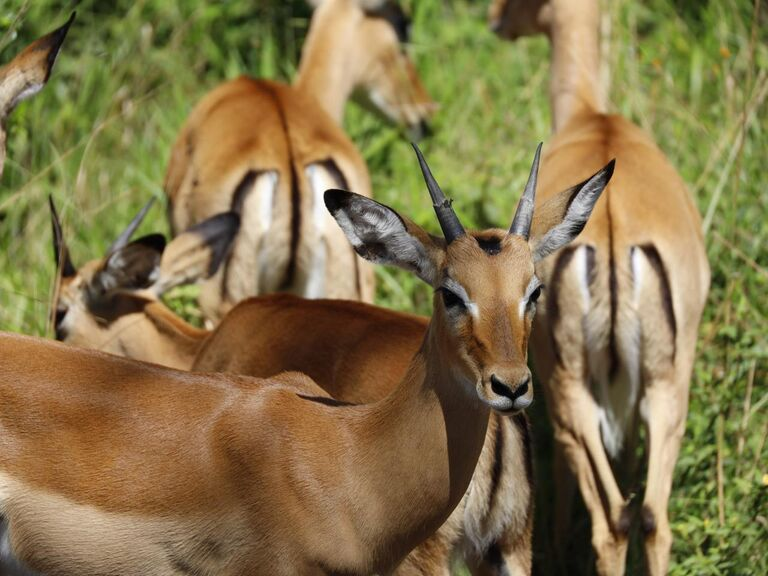
\includegraphics[width=\linewidth]{images/pca_comparison/img_5.lr.jpg}
        \caption*{Input}
    \end{subfigure}\hfill
    \begin{subfigure}{0.195\textwidth}
        \centering
        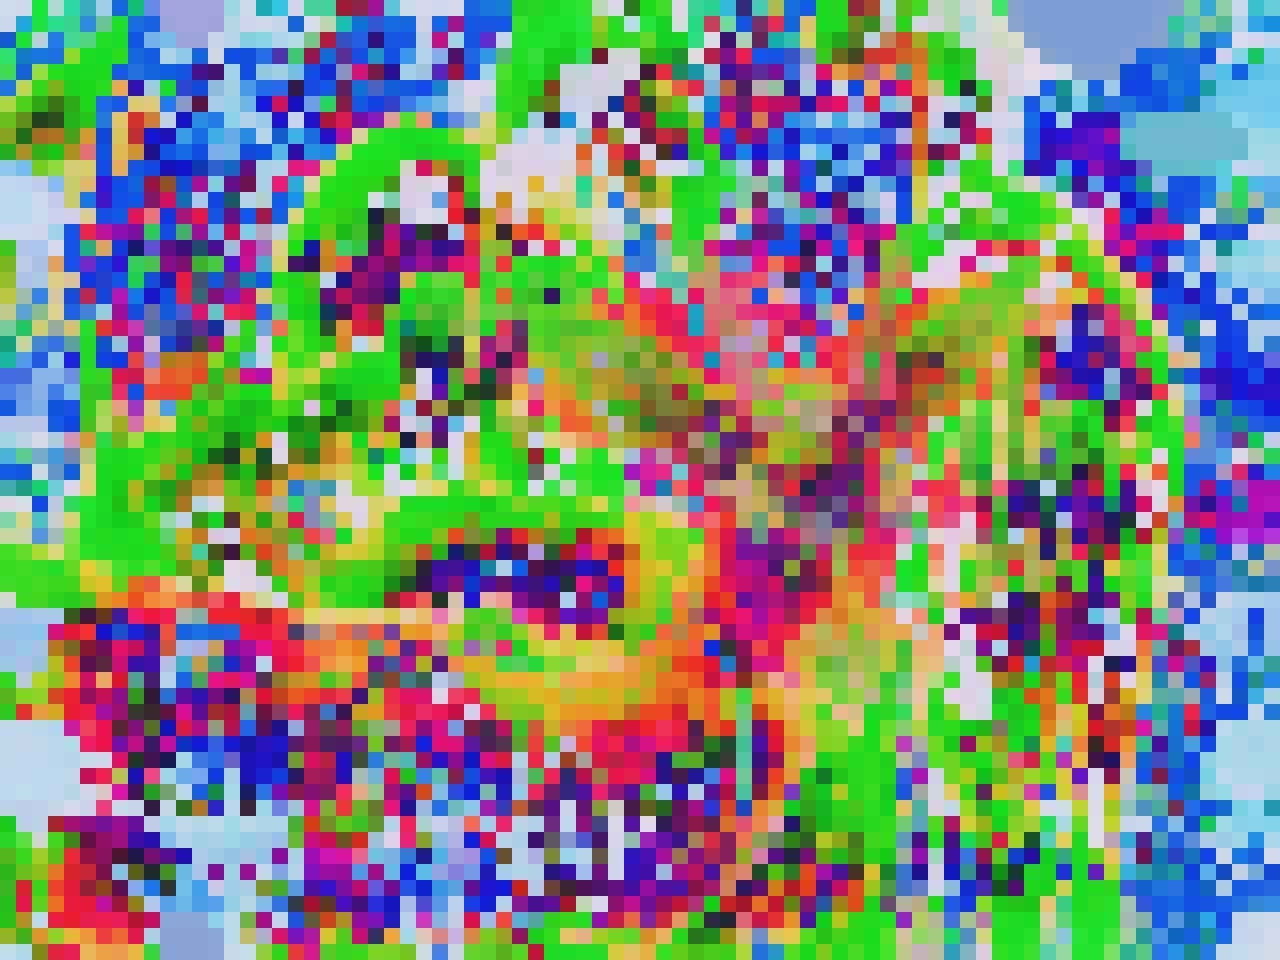
\includegraphics[width=\linewidth]{images/pca_comparison/siglip2/5_m2m1m0.jpg}
        \caption*{SigLIP 2}
    \end{subfigure}\hfill
    \begin{subfigure}{0.195\textwidth}
        \centering
        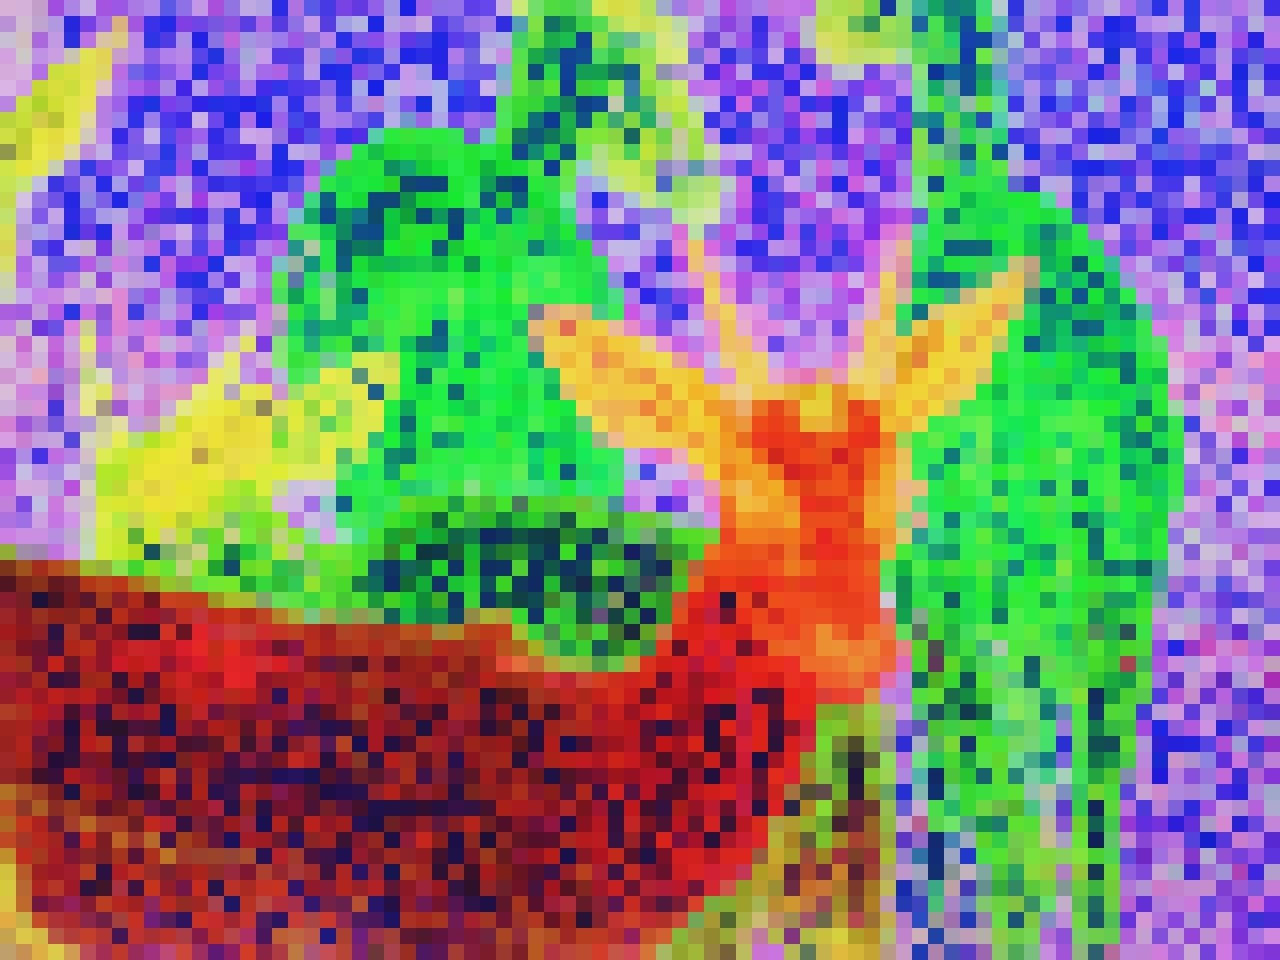
\includegraphics[width=\linewidth]{images/pca_comparison/pe_spatial/5_m2m1p0.jpg}
        \caption*{PE Spatial}
    \end{subfigure}\hfill
    \begin{subfigure}{0.195\textwidth}
        \centering
        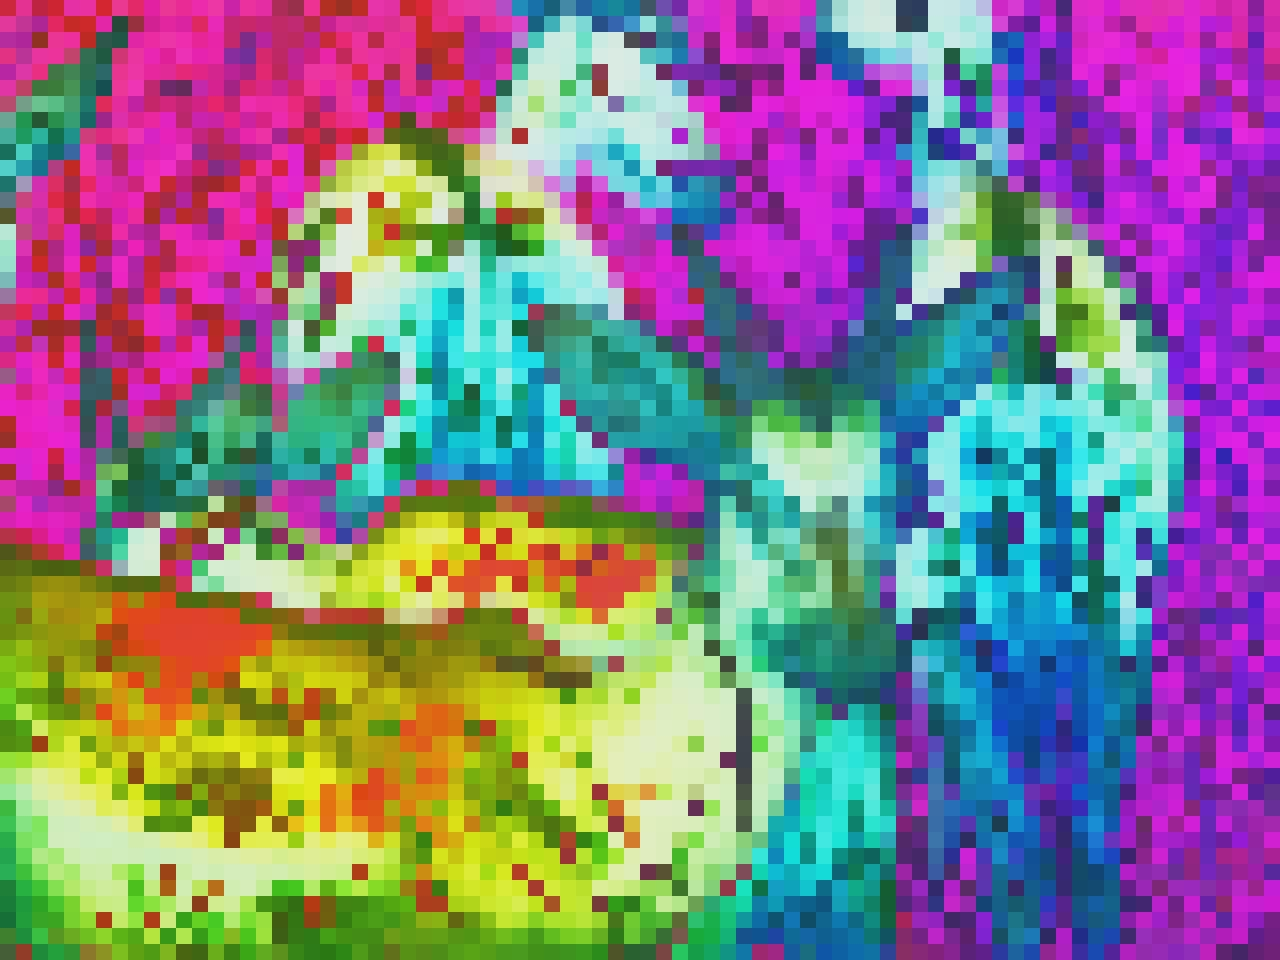
\includegraphics[width=\linewidth]{images/pca_comparison/dinov2/5_m2p0p1.jpg}
        \caption*{DINOv2 w/reg}
    \end{subfigure}\hfill
    \begin{subfigure}{0.195\textwidth}
        \centering
        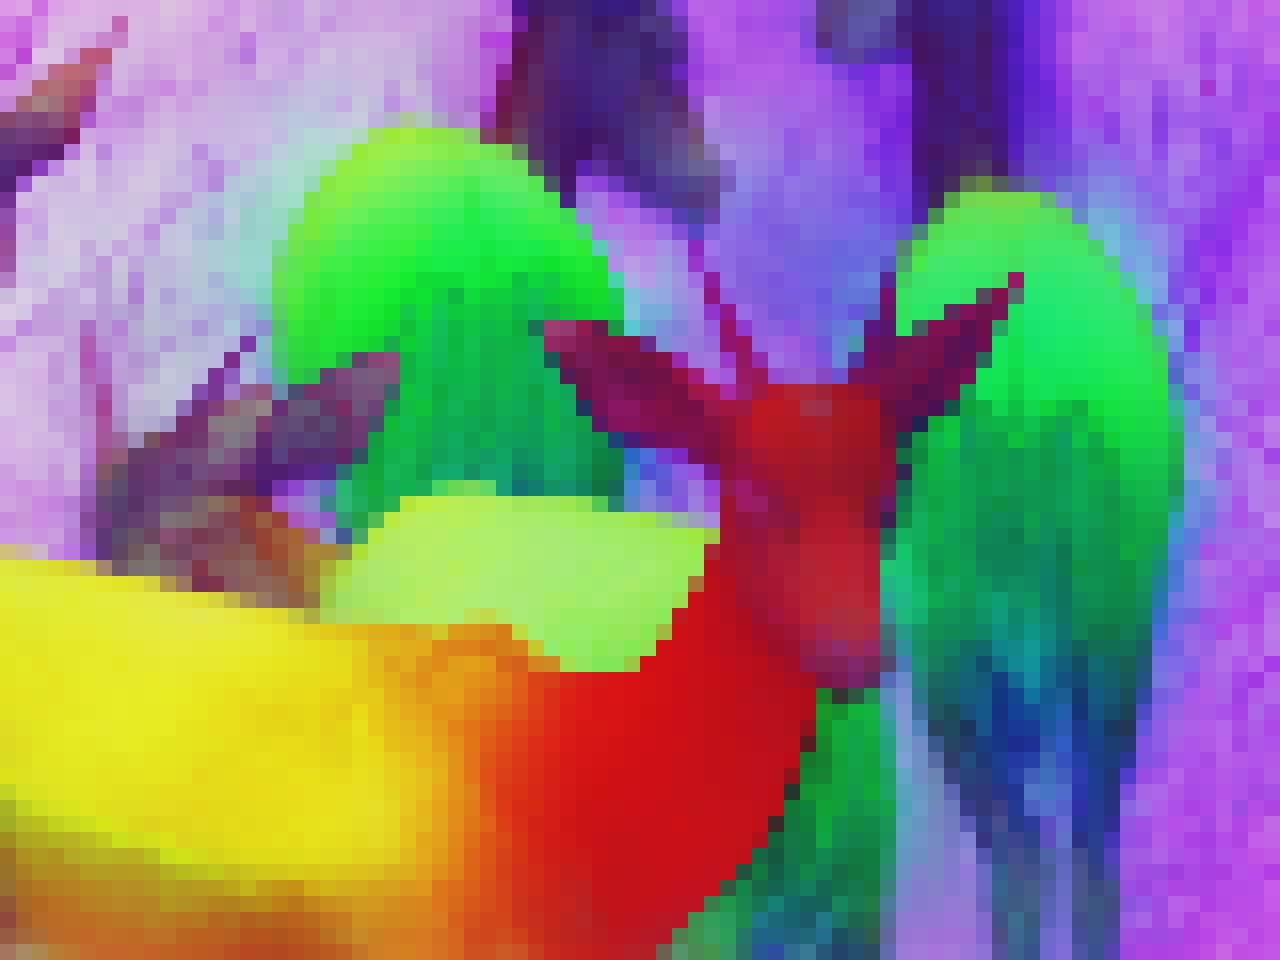
\includegraphics[width=\linewidth]{images/pca_comparison/dinov3/5_m1p2p0.jpg}
        \caption*{DINOv3}
    \end{subfigure}
    \caption{
        Comparison of dense features.
        We compare several vision backbones by projecting their dense outputs using PCA and mapping them to RGB.
        From left to right:
        SigLIP 2 ViT-g/16,
        PEspatial ViT-G/14,
        DINOv2 ViT-g/14 with registers,
        DINOv3 ViT-7B/16.
        Images are forwarded at resolution \(1280{\times}960\) for models using patch 16 and \(1120{\times}840\) for patch 14, \ie all feature maps have size \(80{\times}60\).
    }
    \label{fig:results-pca}
\end{figure}


\subsubsection{Dense Linear Probing}
\label{sec:results-dense-linear-probing}

We perform linear probing on top of the dense features for two tasks: semantic segmentation and monocular depth estimation.
In both cases, we train a linear transform on top of the frozen patch outputs of DINOv3.
For semantic segmentation, we evaluate on the ADE20k~\citep{zhou2017scene}, Cityscapes~\citep{cordts2016cityscapes}, and PASCAL VOC 2012~\citep{pascal-voc-2012} datasets and report the mean intersection-over-union (mIoU) metric.
For depth estimation, we use the NYUv2~\citep{silberman2012indoor} and KITTI~\citep{geiger2013vision} datasets and report the root mean squared error (RMSE).

\begin{table}[t]
    \centering
    \small
    \caption{
        Dense linear probing results on semantic segmentation and monocular depth estimation with frozen backbones. 
        We report the mean Intersection-over-Union (mIoU) metric for the segmentation benchmarks ADE20k, Cityscapes, and VOC. 
        We report the Root Mean Squared Error (RMSE) metric for the depth benchmarks NYUv2 and KITTI. 
        For segmentation, all models are evaluated with input resolution adapted to 1024 patch tokens (\ie $448 \times 448$ for patch size 14, $512 \times 512$ for patch size 16). 
    }
    \label{tab:results-linear-dense}
    \begin{tabular}{@{}ll c ccc c c c @{}}
        \toprule
        & && \multicolumn{3}{c}{Segmentation} && \multicolumn{2}{c}{Depth} \\ 
        \cmidrule{4-6} \cmidrule{8-9}
        Method  & ViT && ADE20k & Citysc. & VOC && NYUv2 $\downarrow$ & KITTI $\downarrow$ \\
        \midrule
        \multicolumn{2}{@{}l}{\resultsTableHeaderAgg} && & && & \\
        AM-RADIOv2.5    & g/14     && 53.0 & 78.4 & 85.4 && 0.340 & 2.918 \\ 
        PEspatial      & G/14     && 49.3 & 73.2 & 82.7 && 0.362 & 3.082 \\
        \midrule
        \multicolumn{2}{@{}l}{\resultsTableHeaderWeakly} && & && & \\
        SigLIP~2        & g/16 && 42.7 & 64.8 & 72.7 && 0.494 & 3.273 \\
        PEcore         & G/14 && 38.9 & 61.1 & 69.2 && 0.590 & 4.119 \\
        \midrule
        \multicolumn{2}{@{}l}{\resultsTableHeaderSelf} && & && & \\
        Franca          & g/14     && 46.3 & 68.7 & 82.9 && 0.445 & 3.140 \\
        DINOv2          & g/14     && 49.5 & 75.6 & 83.1 && 0.372 & 2.624 \\
        Web-DINO        & 7B/14    && 42.7 &  68.3 & 76.1 &&   0.466  &   3.158  \\
        \midrule
        DINOv3          & 7B/16    && \bf 55.9 & \bf 81.1 & \bf 86.6 && \bf 0.309 & \bf 2.346 \\
    \bottomrule
    \end{tabular}
\end{table}

\paragraph[Results]{Results (\cref{tab:results-linear-dense})}
The segmentation results demonstrate the superior quality of our dense features. 
On the general ADE20k dataset, DINOv3 outperforms the self-supervised baselines by more than 6 mIoU points, and the weakly supervised baselines by more than 13 points.
Furthermore, DINOv3 surpasses PEspatial by more than 6 points, and AM-RADIOv2.5 by nearly 3 points. These results are remarkable as both are strong baselines, being distilled from the heavily supervised segmentation model SAM~\citep{kirillov2023segment}.
Similar results are observed on the self-driving benchmark Cityscapes, with DINOv3 achieving the best mIoU of $81.1$, surpassing AM-RADIOv2.5 by 2.5 points, and all other backbones by at least 5.5 points. 

On monocular depth estimation, DINOv3 again outperforms all other models by significant margins: the weakly-supervised models PEcore and SigLIP~2 are still lagging, with DINOv2 and the more advanced models derived from SAM are the closest competitors.
Interestingly, while PEspatial and AM-RADIO show strong performance on NYU, their performance is lower than DINOv2's on KITTI.
Even there, DINOv3 outperforms its predecessor DINOv2 by 0.278 RMSE.

Both sets of evaluations show the outstanding representation power of the dense features of DINOv3 and reflect the visual results from \cref{fig:results-pca}.
With only a linear predictor, DINOv3 allows robust prediction of object categories and masks, as well as physical measurements of the scene such as relative depth.
These results show that the features are not only visually sharp and properly localized, they also represent many important properties of the underlying observations in a linearly separable way.
Finally, the absolute performance obtained with a linear classifier on ADE20k (55.9 mIoU) is itself impressive, as it is not far from the absolute the state-of-the-art (63.0 mIoU) on this dataset.


\subsubsection{3D Correspondence Estimation} 
\label{sec:results-correspondence-estimation}

Understanding the 3D world has always been an important goal of computer vision
Image foundation models have recently fueled research in 3D understanding by offering \emph{3D-aware features}.
In this section, we evaluate the \emph{multi-view consistency} of DINOv3---that is, whether patch features of the same keypoint in different views of an object are similar---following the protocol defined in Probe3D~\citep{banani2024probing}.
We distinguish between \emph{geometric} and \emph{semantic} correspondence estimation. 
The former refers to matching keypoints for the \emph{same object instance} while the latter refers to matching keypoints for different instances of the \emph{same object class}.
We evaluate geometric correspondence on the NAVI dataset~\citep{jampani2023navi} and semantic correspondence on the SPair dataset~\citep{min2019spair71k}, and
measure performance with correspondence recall in both cases.
Please refer to \cref{app:exp-details:keypoint-matching} for more experimental details.


\begin{table}[t]
    \centering
    \small
    \caption{
        Evaluation of 3D consistency of dense representations.
        We estimate 3D keypoint correspondences across views following the evaluation protocol of Probe3D~\citep{banani2024probing}.
        To measure performance, we report the correspondence recall, \ie the percentage of correspondences falling into a specified distance.
    }
    \label{tab:results-correspondence-estimation}
    \begin{tabular}{@{}ll c ccc@{}}
        \toprule
        & && \multicolumn{1}{c}{Geometric} && \multicolumn{1}{c}{Semantic} \\ 
        \cmidrule{4-4} \cmidrule{6-6}
        Method  & ViT && NAVI && SPair \\
        \midrule
        \multicolumn{2}{@{}l}{\resultsTableHeaderAgg} && & \\
        AM-RADIOv2.5    & g/14   && 59.4 && 56.8 \\ 
        PEspatial      & G/14   && 53.8 && 49.6 \\
        \midrule
        \multicolumn{2}{@{}l}{\resultsTableHeaderWeakly} && & \\
        SigLIP~2        & g/16   && 49.4 && 42.6 \\
        PEcore         & G/14   && 39.9 && 23.1 \\
        \midrule
        \multicolumn{2}{@{}l}{\resultsTableHeaderSelf} && & \\
        Franca          & g/14   && 54.6 && 51.0 \\
        DINOv2          & g/14   && 60.1 && 56.1 \\
        Web-DINO        & 7B/14  && 55.0 && 32.2 \\        
        \midrule
        DINOv3          & 7B/16  && \bf 64.4 && \bf 58.7 \\
    \bottomrule
    \end{tabular}
\end{table}

\paragraph[Results]{Results (\cref{tab:results-correspondence-estimation})}
For geometric correspondences, DINOv3 outperforms all other models and improves over the second best model (DINOv2) by 4.3\% recall.
Other SSL scaling endeavors (Franca and WebSSL) lag behind DINOv2, showing that it is still a strong baseline.
Weakly-supervised models (PEcore and SigLIP~2) do not fare well on this task, indicating a lack of 3D awareness. 
For models with SAM distillation, AM-RADIO nearly reaches the performance of DINOv2, but PEspatial still lags behind it ($-11.6$\% recall), and even falls behind Franca ($-0.8$\% recall).
This suggests that self-supervised learning is a key component for strong performance on this task.
For semantic correspondences, the same conclusions apply.
DINOv3 performs best, outperforming both its predecessor ($+2.6$\% recall) and AM-RADIO ($+1.9$\% recall).
Overall, these impressive performance on keypoint matching are very promising signals for downstream use of DINOv3 in other 3D-heavy applications. 


\subsubsection{Unsupervised Object Discovery}
\label{sec:results-object-discovery}

Powerful self-supervised features facilitate discovering object instances in images without requiring \emph{any} annotations~\citep{Vo21LOD,simeoni2021localizing,seitzer2023bridging,wang2023tokencut,simeoni2025unsupervised}. 
We test this capability for different vision encoders via the task of unsupervised object discovery, which requires class-agnostic segmentation of objects in images~\citep{Russell06ObjectDiscovery,tuytelaars2010bjectDiscovery,Cho2015ObjectDiscovery,Vo2019UnsupOptim}.
In particular, we use the non-parametric graph-based TokenCut algorithm~\citep{wang2023tokencut}, which has shown strong performance on a variety of backbones.
We run it on three widely used datasets: VOC 2007, VOC 2012~\citep{everingham2015pascal}, and COCO-20k~\citep{Lin2014cocodataset,Vo20rOSD}. 
We follow the evaluation protocol defined by \citet{simeoni2021localizing} and report the CorLoc metric. 
To properly compare backbones with different feature distributions, we perform a search over the main TokenCut hyperparameter, namely the cosine similarity threshold applied when constructing the patch graph used for partitioning. 
Originally, the best object discovery results were obtained with DINO~\citep{caron2021emerging} using the keys of the last attention layer.
However, this hand-crafted choice does not consistently generalize to other backbones.
For simplicity, we always employ the output features for all models. 

\paragraph[Results]{Results (\cref{tab:results-object-discovery})}
The original DINO has set a very high bar for this task. 
Interestingly, while DINOv2 has shown very strong performance for pixel-wise dense tasks, it fails at object discovery.
This can in part be attributed to the artifacts present in the dense features (\cf \cref{fig:results-pca}).
DINOv3, with its clean and precise output feature maps outperforms both its predecessors, with a $5.9$ CorLoc improvement on VOC 2007, and all other backbones, whether self-, weakly-supervised or agglomerative.
This evaluation confirms that DINOv3's dense features are both semantically strong and well localized.
We believe that this will pave the way for more class-agnostic object detection approaches, especially in scenarios where annotations are costly or unavailable, and where the set of relevant classes is not confined to a predefined subset.

\begin{figure}[t]
    \centering
    \small
    \begin{minipage}{0.57\textwidth}
        \begin{tabular}{@{}ll c ccc@{}}
            \toprule
            Method & ViT & & VOC07 & VOC12 & COCO \\
            \midrule
            \multicolumn{2}{@{}l}{\resultsTableHeaderAgg} && & \\
            AM-RADIOv2.5    & g/14     && 55.0 & 59.7 & 45.9 \\ 
            PEspatial      & G/14     && 51.2 & 56.0 & 43.9 \\
            \midrule
            \multicolumn{2}{@{}l}{\resultsTableHeaderWeakly} && & \\
            SigLIPv2        & g/16     && 20.5 &  24.7 & 18.6 \\
            PEcore         & G/14     && 14.2 & 18.2 & 13.5 \\
            \midrule
            \multicolumn{2}{@{}l}{\resultsTableHeaderSelf} && & \\
            DINO            & S/16     && 61.1 & 66.0 & 48.7 \\
            DINO            & B/16     && 60.1 & 64.4 & 50.5 \\
            DINOv2          & g/14     && 55.6 & 60.4 & 45.4 \\
            Web-DINO        & 7B/14    && 26.1 & 29.7 & 20.9 \\
            \midrule
            DINOv3          & 7B/16    && \bf 66.1 & \bf 69.5 & \bf 55.1 \\
            \bottomrule
        \end{tabular}
    \end{minipage}
    \hfill
    \begin{minipage}{0.42\textwidth}
    \raisebox{-3em}{
    \renewcommand{\arraystretch}{0.2}
    \setlength{\tabcolsep}{0.3pt}
    \begin{tabular}{cc}
       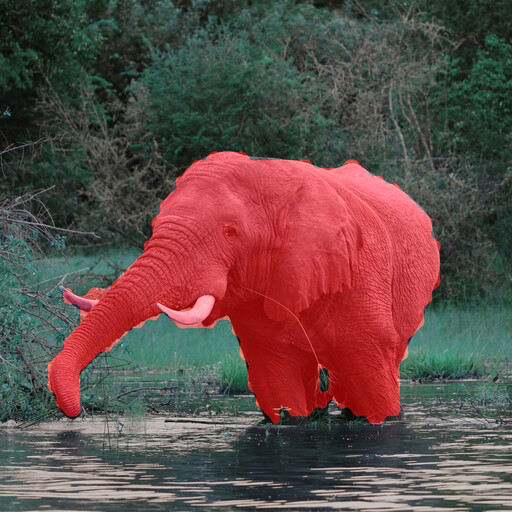
\includegraphics[width=0.42\linewidth]{images/tokencut/tokencut_m4_bright.lr.JPG}   &   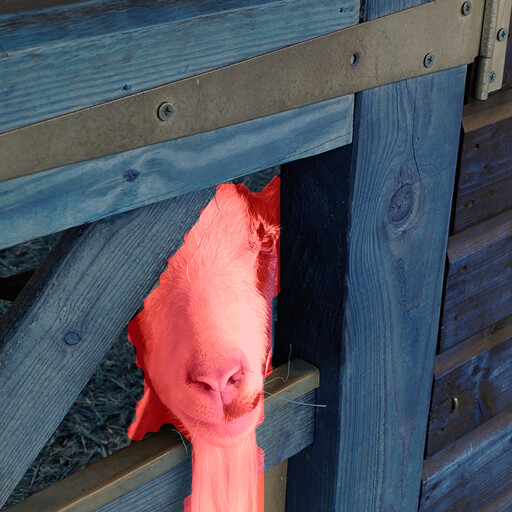
\includegraphics[width=0.42\linewidth]{images/tokencut/tokencut_P_20240712_124515_bright.lr.jpg} \\
        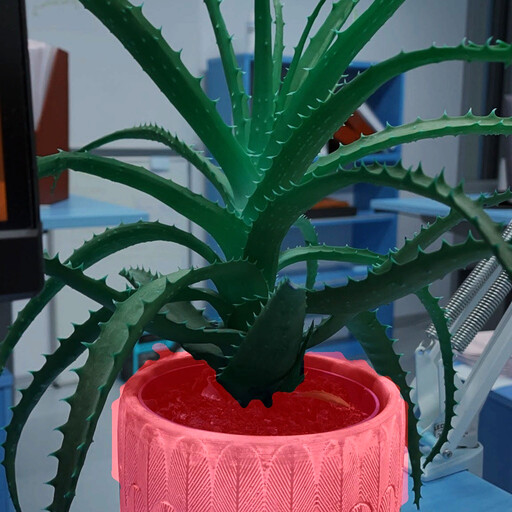
\includegraphics[width=0.42\linewidth]{images/tokencut/tokencut_IMG-20210916-WA0019_bright.lr.jpg} &  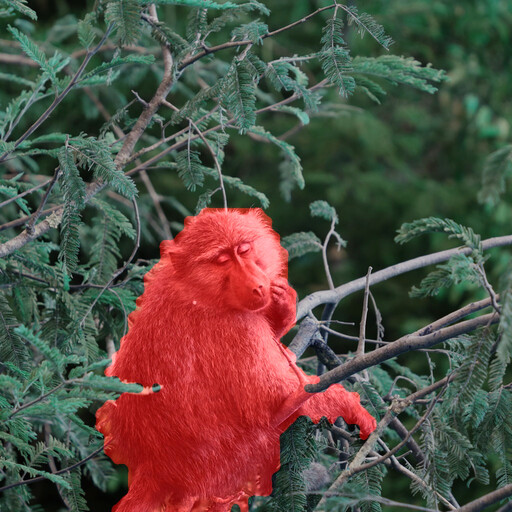
\includegraphics[width=0.42\linewidth]{images/tokencut/tokencut_m7_bright.lr.JPG}
    \end{tabular}
    }
    \end{minipage}
    \caption{
        Unsupervised object discovery.
        We apply TokenCut~\citep{wang2022self} on the output patch features of different backbones and report CorLoc metric. We also visualize predicted masks obtained with DINOv3 (red overlay on input images at res. $1024$), obtained \emph{with no annotation and no post-processing}.
    }
    \label{tab:results-object-discovery}
\end{figure}

\subsubsection{Video Segmentation Tracking}
\label{sec:results-tracking}

Beyond static images, an important property of visual representations is their \emph{temporal consistency}, \ie whether the features evolve in a stable manner through time.
To test for this property, we evaluate DINOv3 on the task of video segmentation tracking: given ground-truth instance segmentation masks in the first frame of a video, the goal is to propagate these masks to subsequent frames.
We use the DAVIS~2017~\citep{pont20172017}, YouTube-VOS~\citep{xu2018youtubevos}, and MOSE~\citep{ding2023mose} datasets.
We evaluate performance using the standard \(\JnF\)-mean metric, which combines region similarity (\(\mathcal{J}\)) and contour accuracy (\(\mathcal{F}\))~\citep{perazzi2016benchmark}.
Following \citet{jabri2020space}, we use a non-parametric label propagation algorithm that considers the similarity between patch features across frames.
We evaluate at three input resolutions, using a short side length of 420/480 (S), 840/960 (M), and 1260/1440 (L) pixels for models with patch size 14/16 (matching the number of patch tokens).
The \(\JnF\) score is always computed at the native resolution of the videos.
See \cref{app:exp-details:tracking} for more detailed experimental settings.

\begin{table}[t]
    \centering
    \small
    \caption{
        Video segmentation tracking evaluation.
        We report the \(\JnF\)-mean on DAVIS, YouTube-VOS, and MOSE at multiple resolutions.
        For models with patch size 14/16, the small, medium and large resolutions correspond to a video short side of 420/480, 840/960, 1260/1140 pixels.
    }
    \label{tab:results-video-segmentation-tracking}
    \begin{tabular}{@{}ll ccc ccc ccc@{}}
        \toprule
        & & \multicolumn{3}{c}{DAVIS} & \multicolumn{3}{c}{YouTube-VOS} & \multicolumn{3}{c}{MOSE} \\
        \cmidrule(lr){3-5} \cmidrule(lr){6-8} \cmidrule(lr){9-11}
        Method & ViT & S & M & L & S & M & L & S & M & L \\
        \midrule
        \multicolumn{2}{@{}l}{\resultsTableHeaderAgg} & & & & & & & & & \\
        AM-RADIOv2.5    & g/14  & 66.5 & 77.3 & 81.4 & 70.1 & 78.1 & 79.2 & 44.0 & 52.6 & 54.3 \\
        PEspatial      & G/14  & 68.4 & 74.5 & 70.5 & 68.5 & 67.5 & 55.6 & 39.3 & 40.2 & 34.0 \\
        \midrule
        \multicolumn{2}{@{}l}{\resultsTableHeaderWeakly} & & & & & & & & & \\
        SigLIP 2        & g/16  & 56.1 & 62.3 & 62.9 & 52.0 & 57.3 & 55.1 & 28.0 & 30.3 & 29.2 \\
        PEcore         & G/14  & 48.2 & 53.1 & 49.8 & 34.7 & 33.0 & 25.3 & 17.8 & 19.0 & 15.4 \\
        \midrule
        \multicolumn{2}{@{}l}{\resultsTableHeaderSelf} & & & & & & & & & \\
        Franca          & g/14  & 61.8 & 66.9 & 66.5 & 67.3 & 70.5 & 67.9 & 40.3 & 42.6 & 41.9 \\
        DINOv2          & g/14  & 63.9 & 73.6 & 76.6 & 65.6 & 73.5 & 74.6 & 40.4 & 47.6 & 48.5 \\
        Web-DINO        & 7B/14 & 57.2 & 65.8 & 69.5 & 43.9 & 49.6 & 50.9 & 24.9 & 29.9 & 31.1 \\
        \midrule
        DINOv3          & 7B/16  & \bf 71.1 & \bf 79.7 & \bf 83.3 & \bf 74.1 & \bf 80.2 & \bf 80.7 & \bf 46.0 & \bf 53.9 & \bf 55.6 \\
        \bottomrule
    \end{tabular}
\end{table}

\paragraph[Results]{Results (\cref{tab:results-video-segmentation-tracking})} 
Aligned with all previous results, weakly-supervised backbones do not deliver convincing performance. 
PEspatial, distilled from the video model SAMv2, provides satisfactory performance, surpassing DINOv2 on smaller resolutions, but falling short on larger ones.
Across resolutions, DINOv3 outperforms all competitors, with a staggering $83.3$ $\JnF$ on DAVIS-L, $6.7$ points above DINOv2.
Furthermore, performance as a function of resolution follows a healthy trend, confirming that our model is able to make use of more input pixels to output precise, high-resolution feature maps (\cf \cref{fig:intro:dense-quality,fig:visualization-extreme-resolutions}).
In contrast, performance at higher resolutions stays almost flat for SigLIP~2 and PEcore, and degrades for PEspatial.
Interestingly, our image model, without any tuning on video, allows to properly track objects in time (see \cref{fig:segmentation-tracking-example}).
This makes it a great candidate to embed videos, allowing to build strong video models on top.

\begin{figure}[t]
    \centering
    \begin{subfigure}[b]{0.195\textwidth}
        \centering
        
\includegraphics[width=\textwidth]{images/segmentation_tracking/ducks/rgb_frames/000001.jpg}
    \end{subfigure}\hfill
    \begin{subfigure}[b]{0.195\textwidth}
        \centering
        
\includegraphics[width=\textwidth]{images/segmentation_tracking/ducks/rgb_frames/000031.jpg}
    \end{subfigure}\hfill
    \begin{subfigure}[b]{0.195\textwidth}
        \centering
        
\includegraphics[width=\textwidth]{images/segmentation_tracking/ducks/rgb_frames/000061.jpg}
    \end{subfigure}\hfill
    \begin{subfigure}[b]{0.195\textwidth}
        \centering
        
\includegraphics[width=\textwidth]{images/segmentation_tracking/ducks/rgb_frames/000091.jpg}
    \end{subfigure}\hfill
    \begin{subfigure}[b]{0.195\textwidth}
        \centering
        
\includegraphics[width=\textwidth]{images/segmentation_tracking/ducks/rgb_frames/000121.jpg}
    \end{subfigure}\vspace{0.25em}
    \begin{subfigure}[b]{0.195\textwidth}
        \centering
        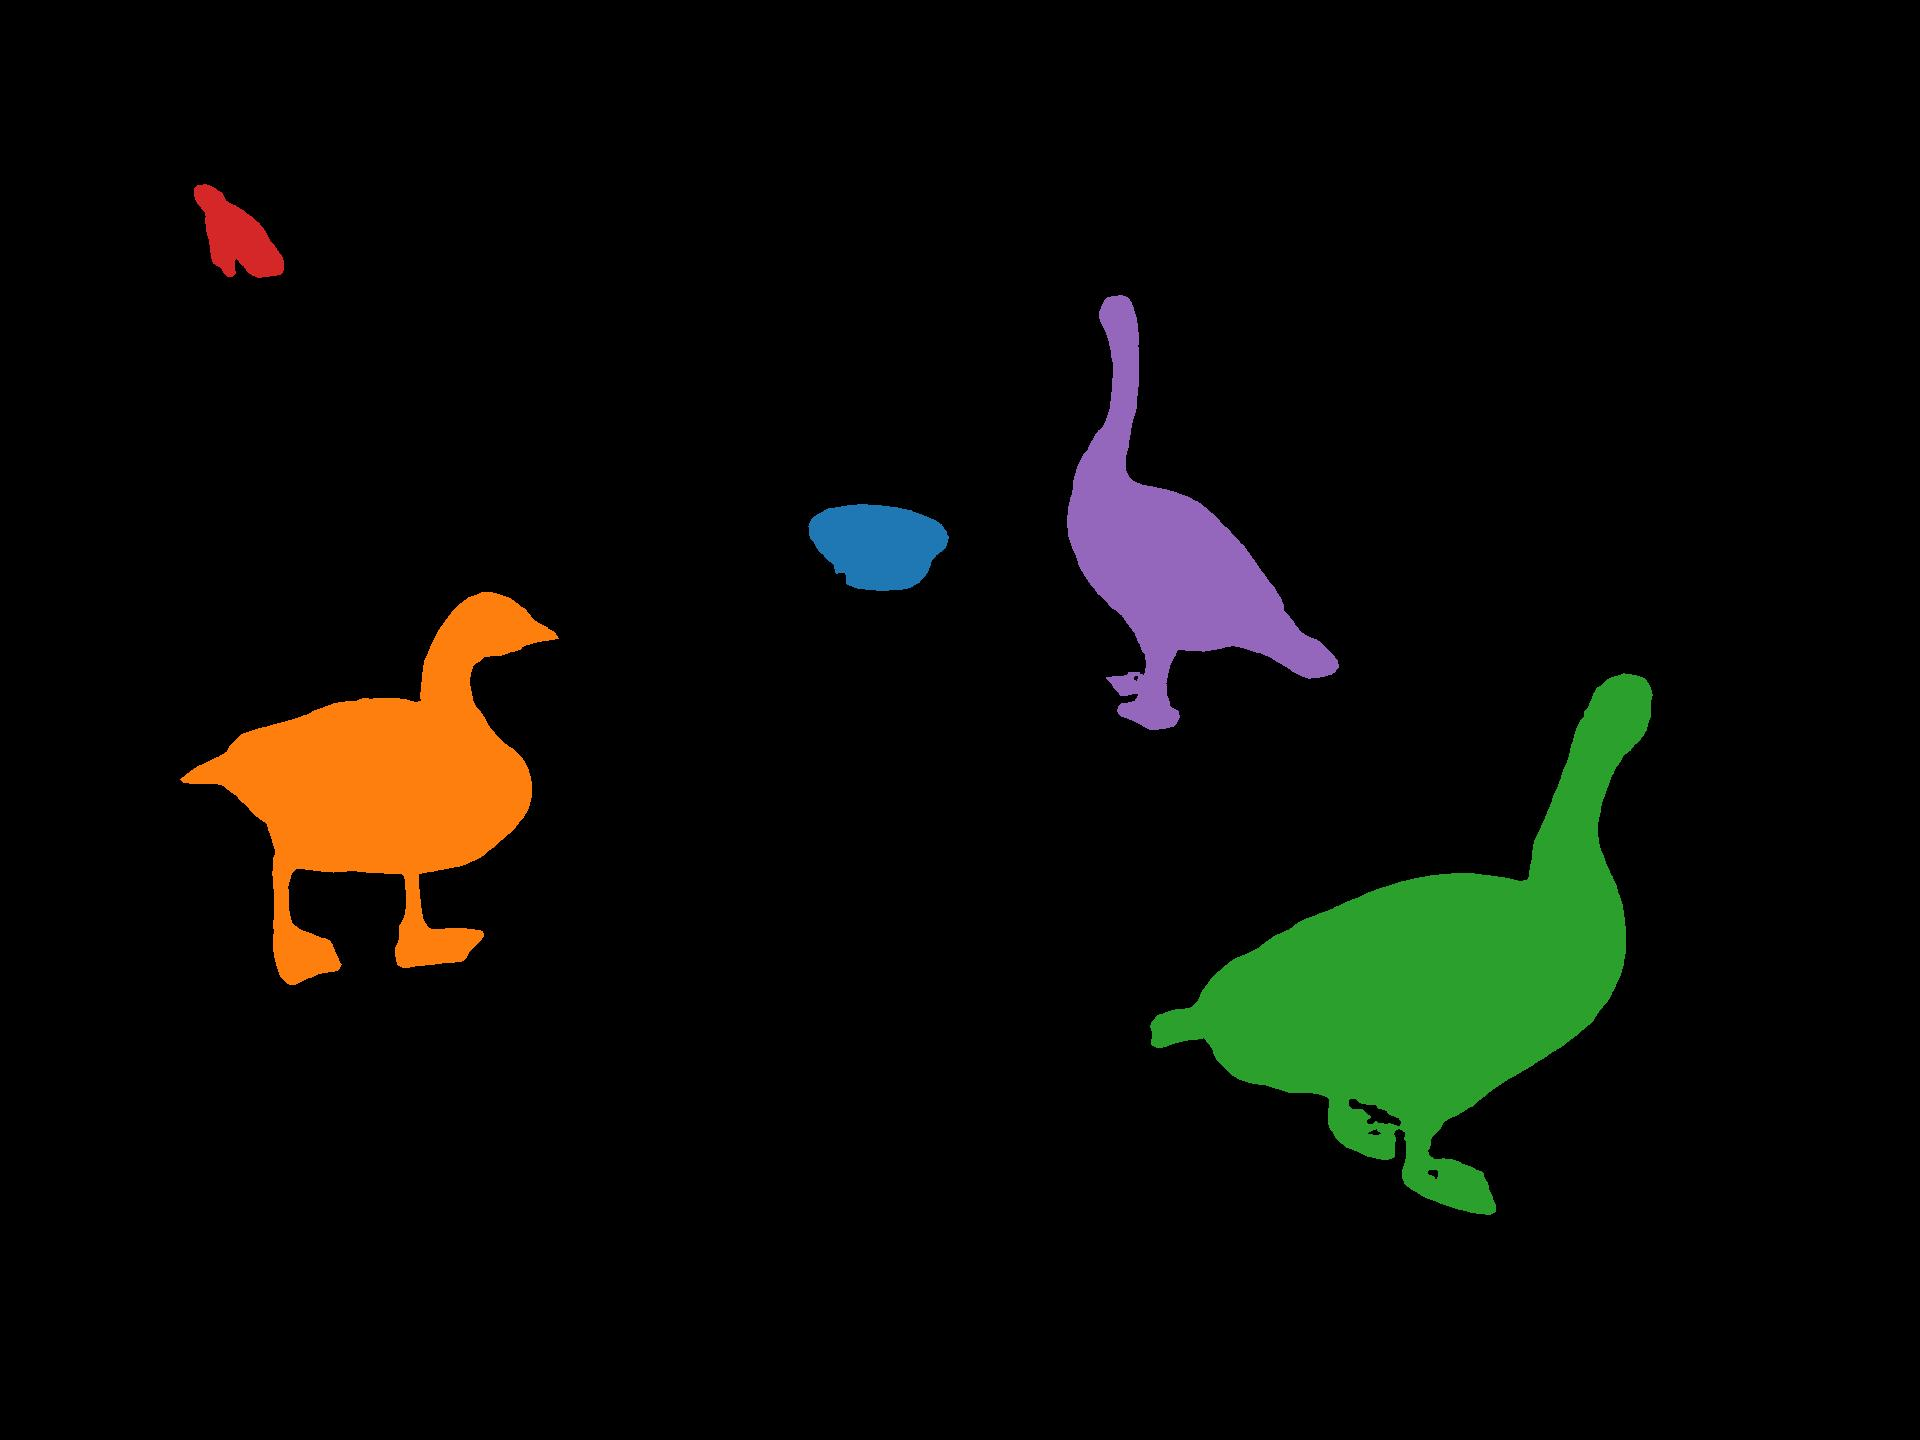
\includegraphics[width=\textwidth]{images/segmentation_tracking/ducks/all_obj/000001.jpg}
        \caption*{Initial frame}
    \end{subfigure}\hfill
    \begin{subfigure}[b]{0.195\textwidth}
        \centering
        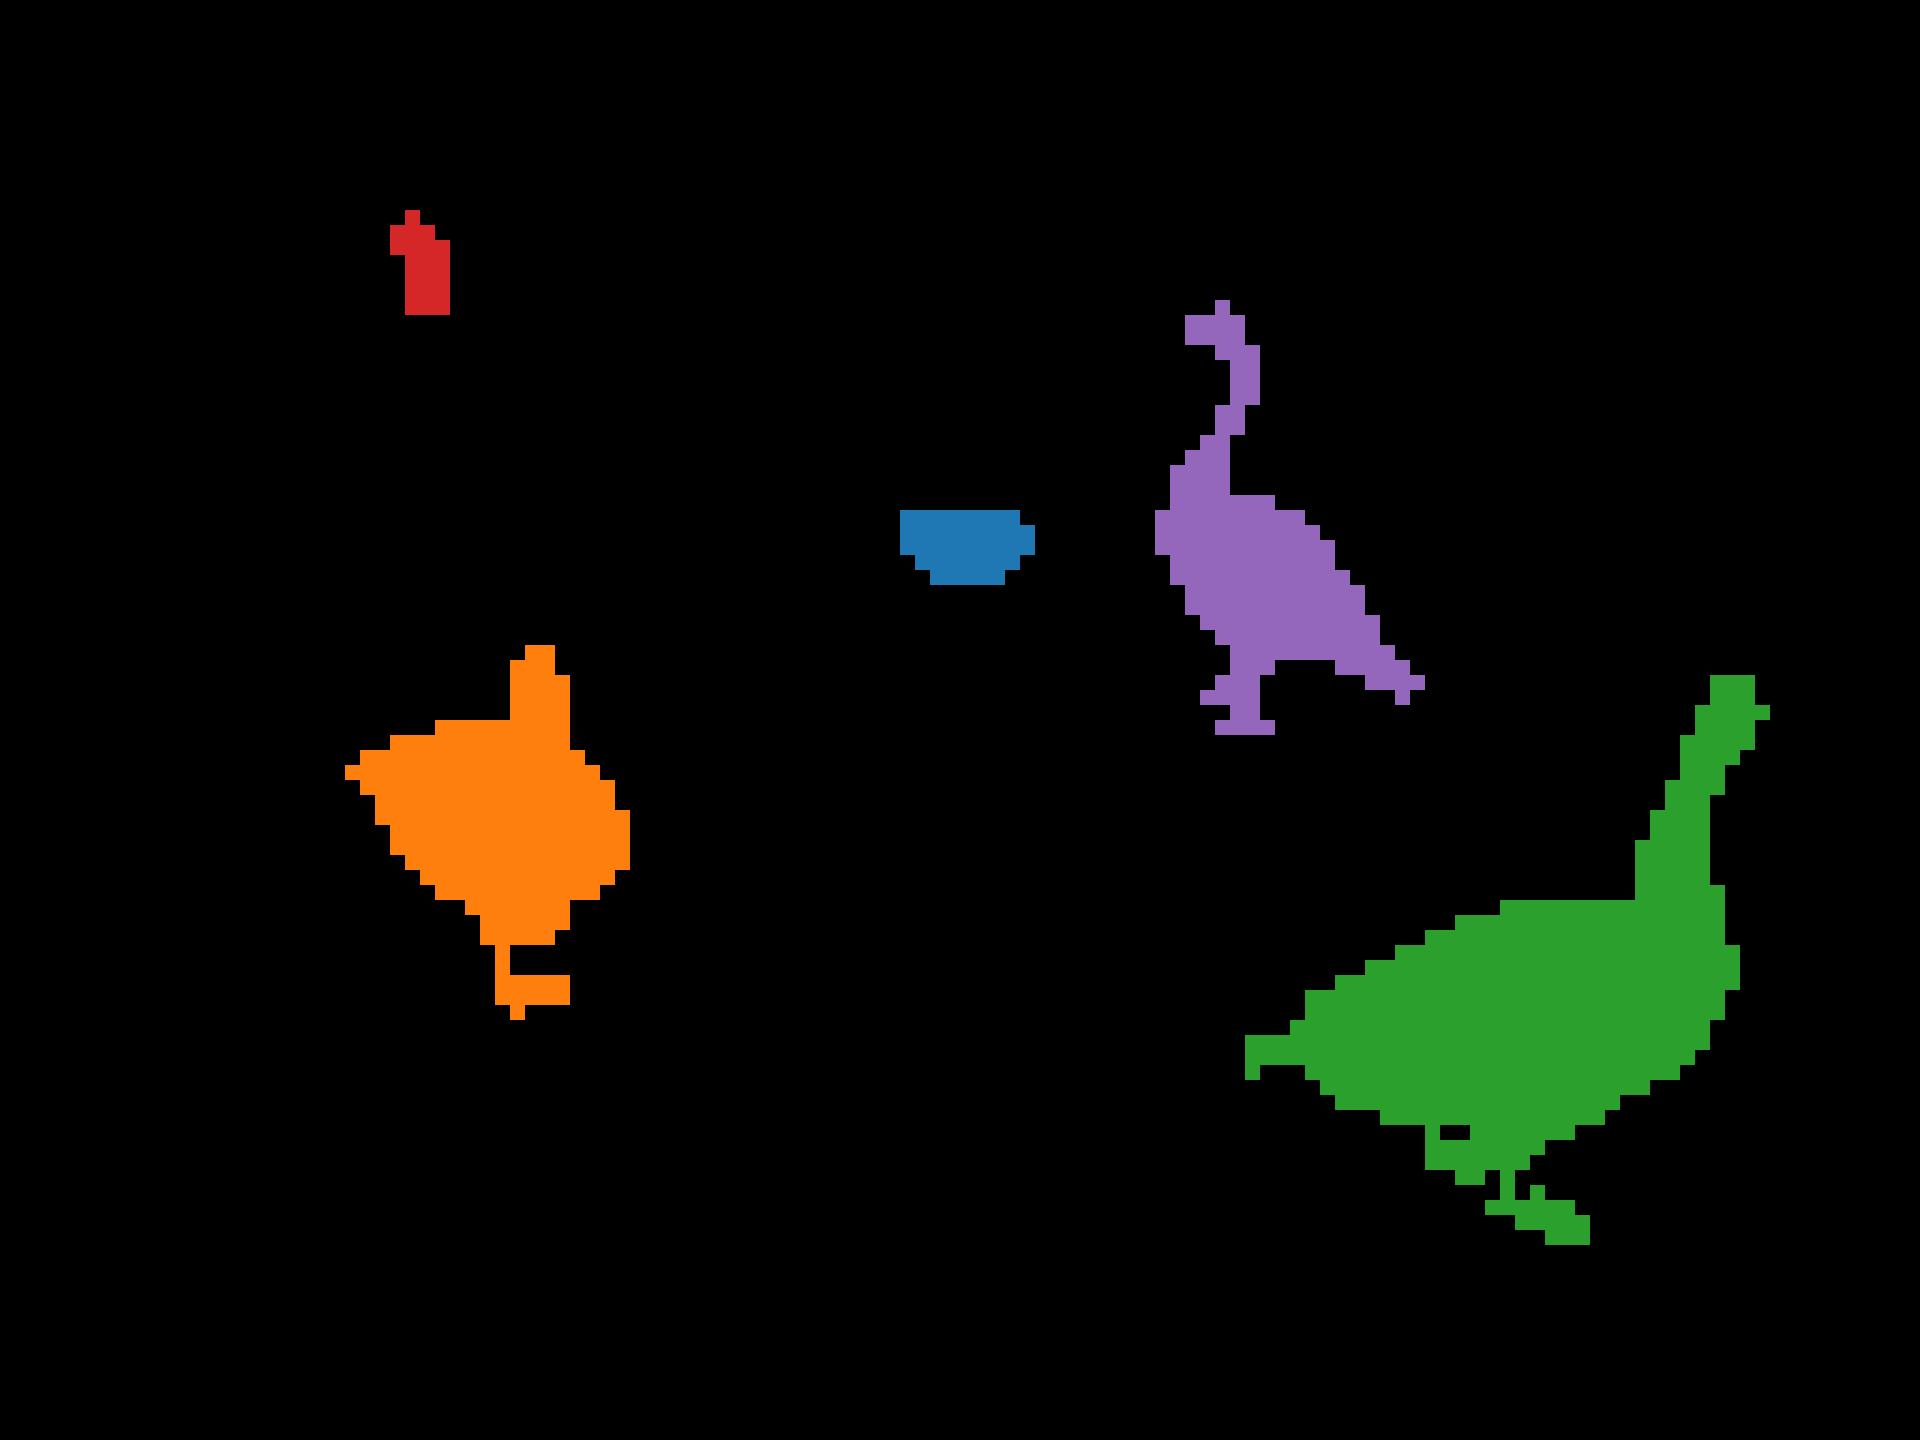
\includegraphics[width=\textwidth]{images/segmentation_tracking/ducks/all_obj/000031.jpg}
        \caption*{Frame 30}
    \end{subfigure}\hfill
    \begin{subfigure}[b]{0.195\textwidth}
        \centering
        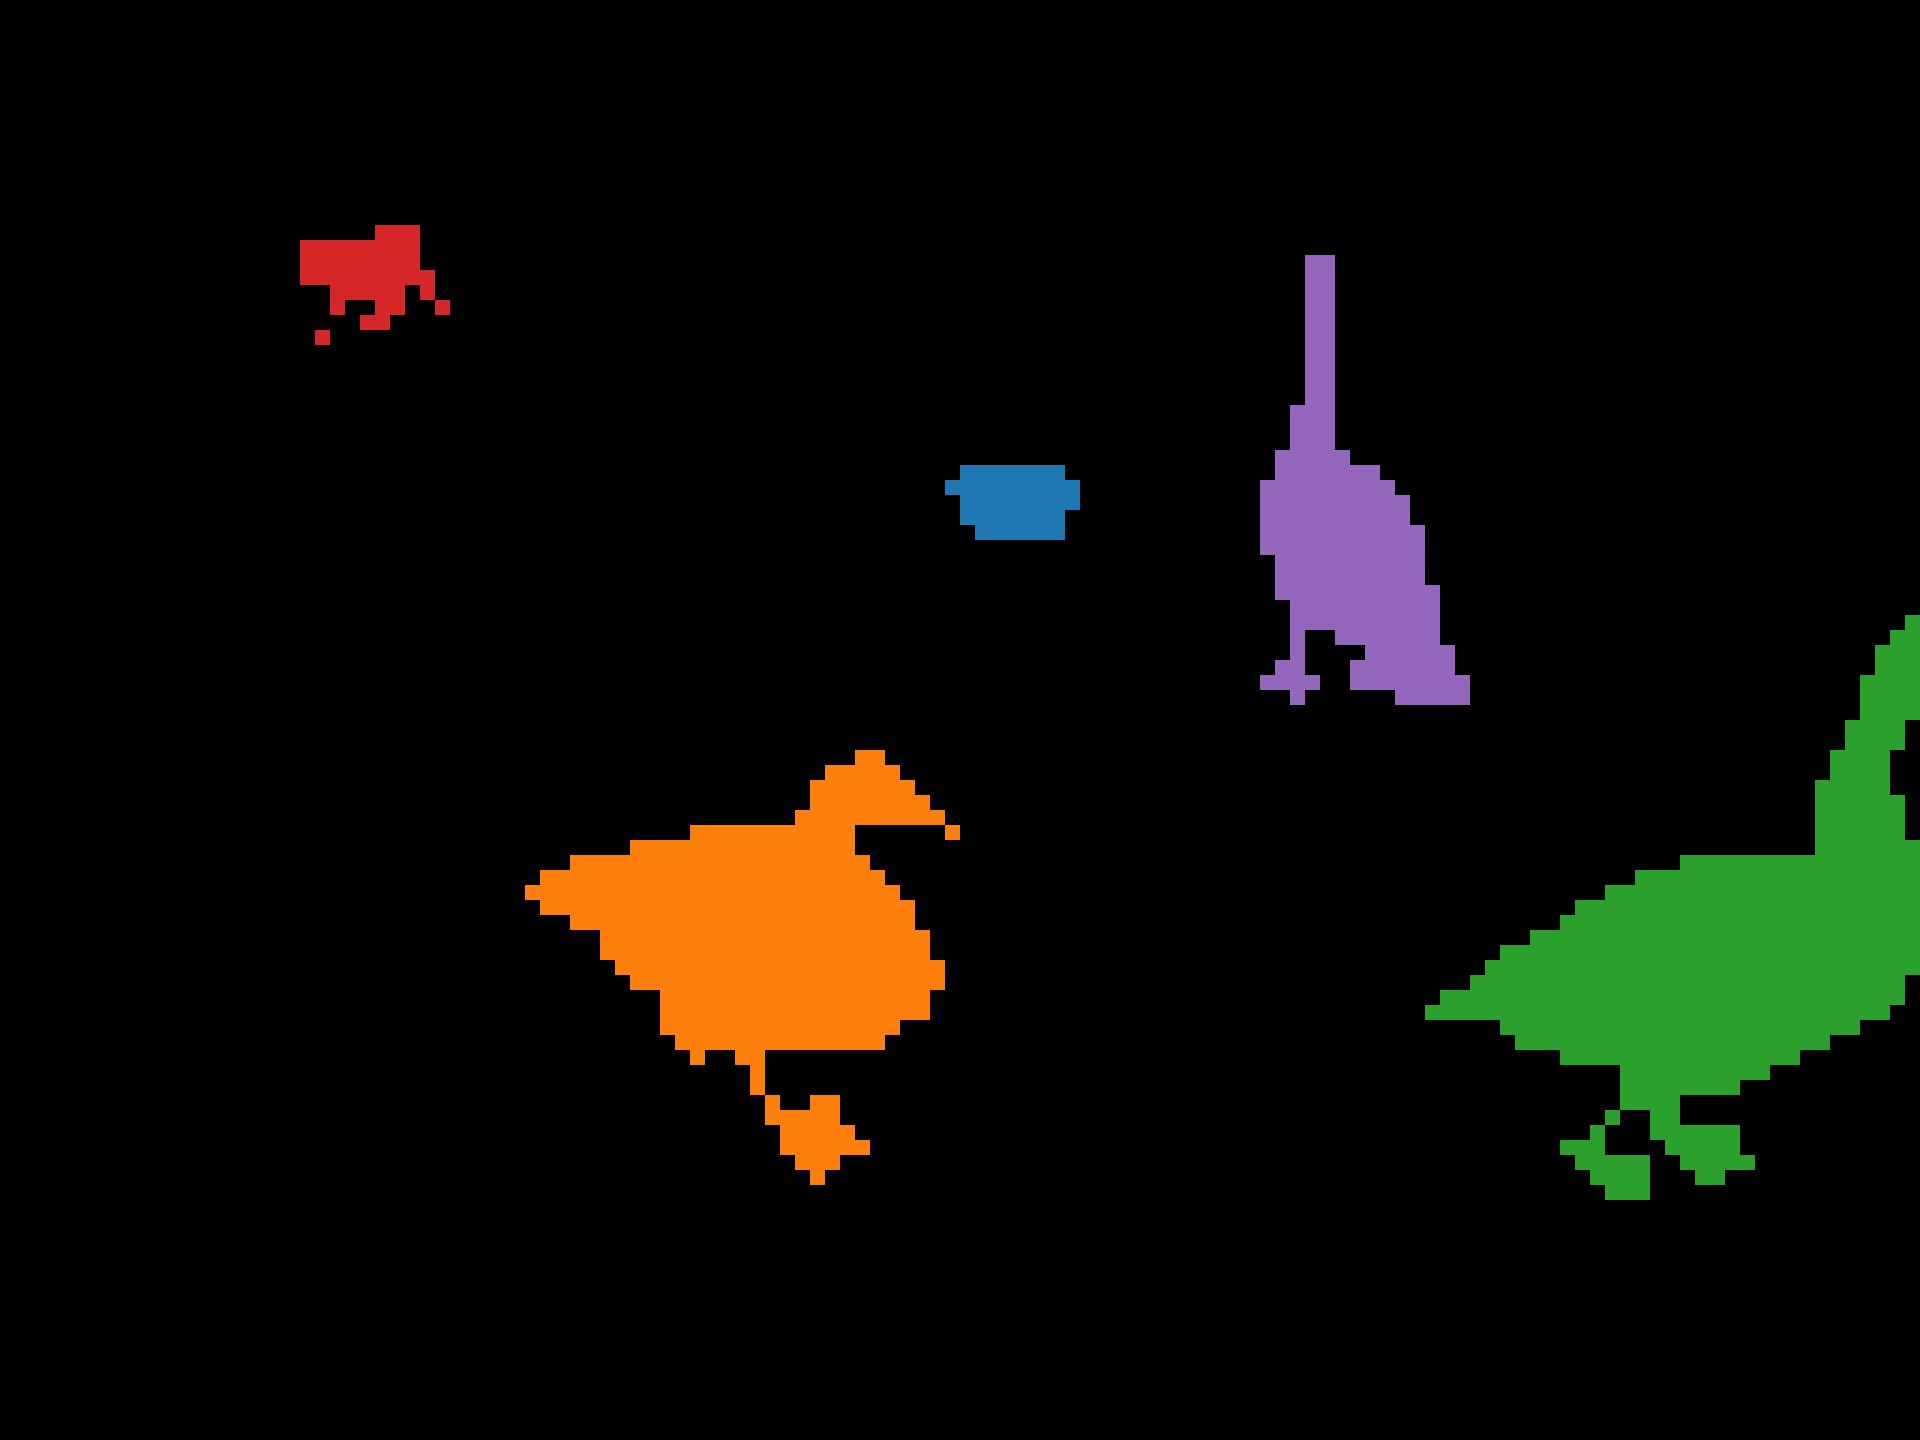
\includegraphics[width=\textwidth]{images/segmentation_tracking/ducks/all_obj/000061.jpg}
        \caption*{Frame 60}
    \end{subfigure}\hfill
    \begin{subfigure}[b]{0.195\textwidth}
        \centering
        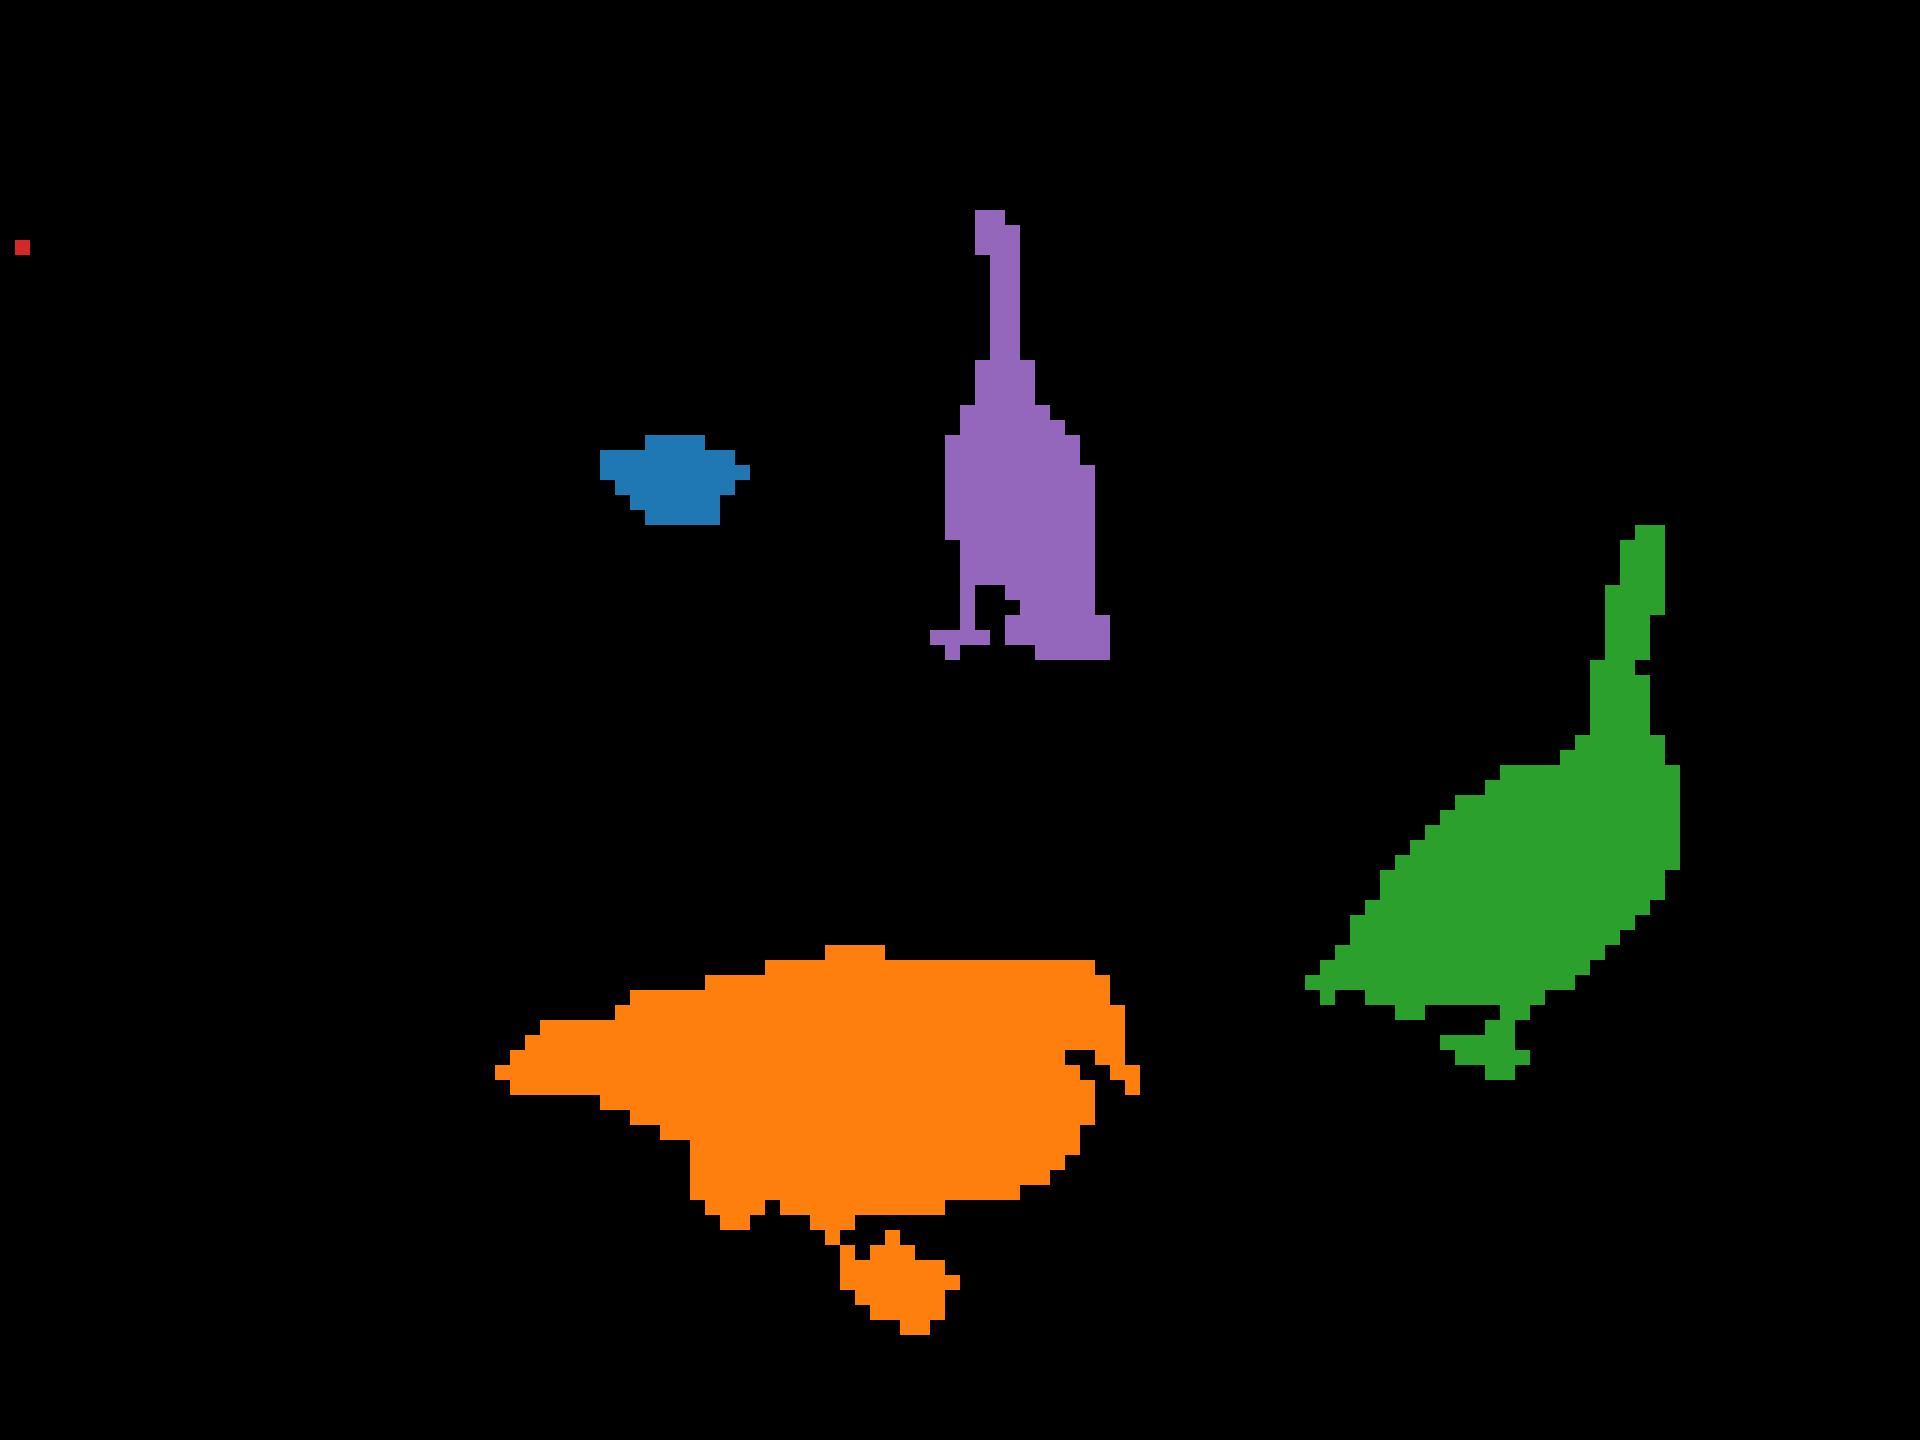
\includegraphics[width=\textwidth]{images/segmentation_tracking/ducks/all_obj/000091.jpg}
        \caption*{Frame 90}
    \end{subfigure}\hfill
    \begin{subfigure}[b]{0.195\textwidth}
        \centering
        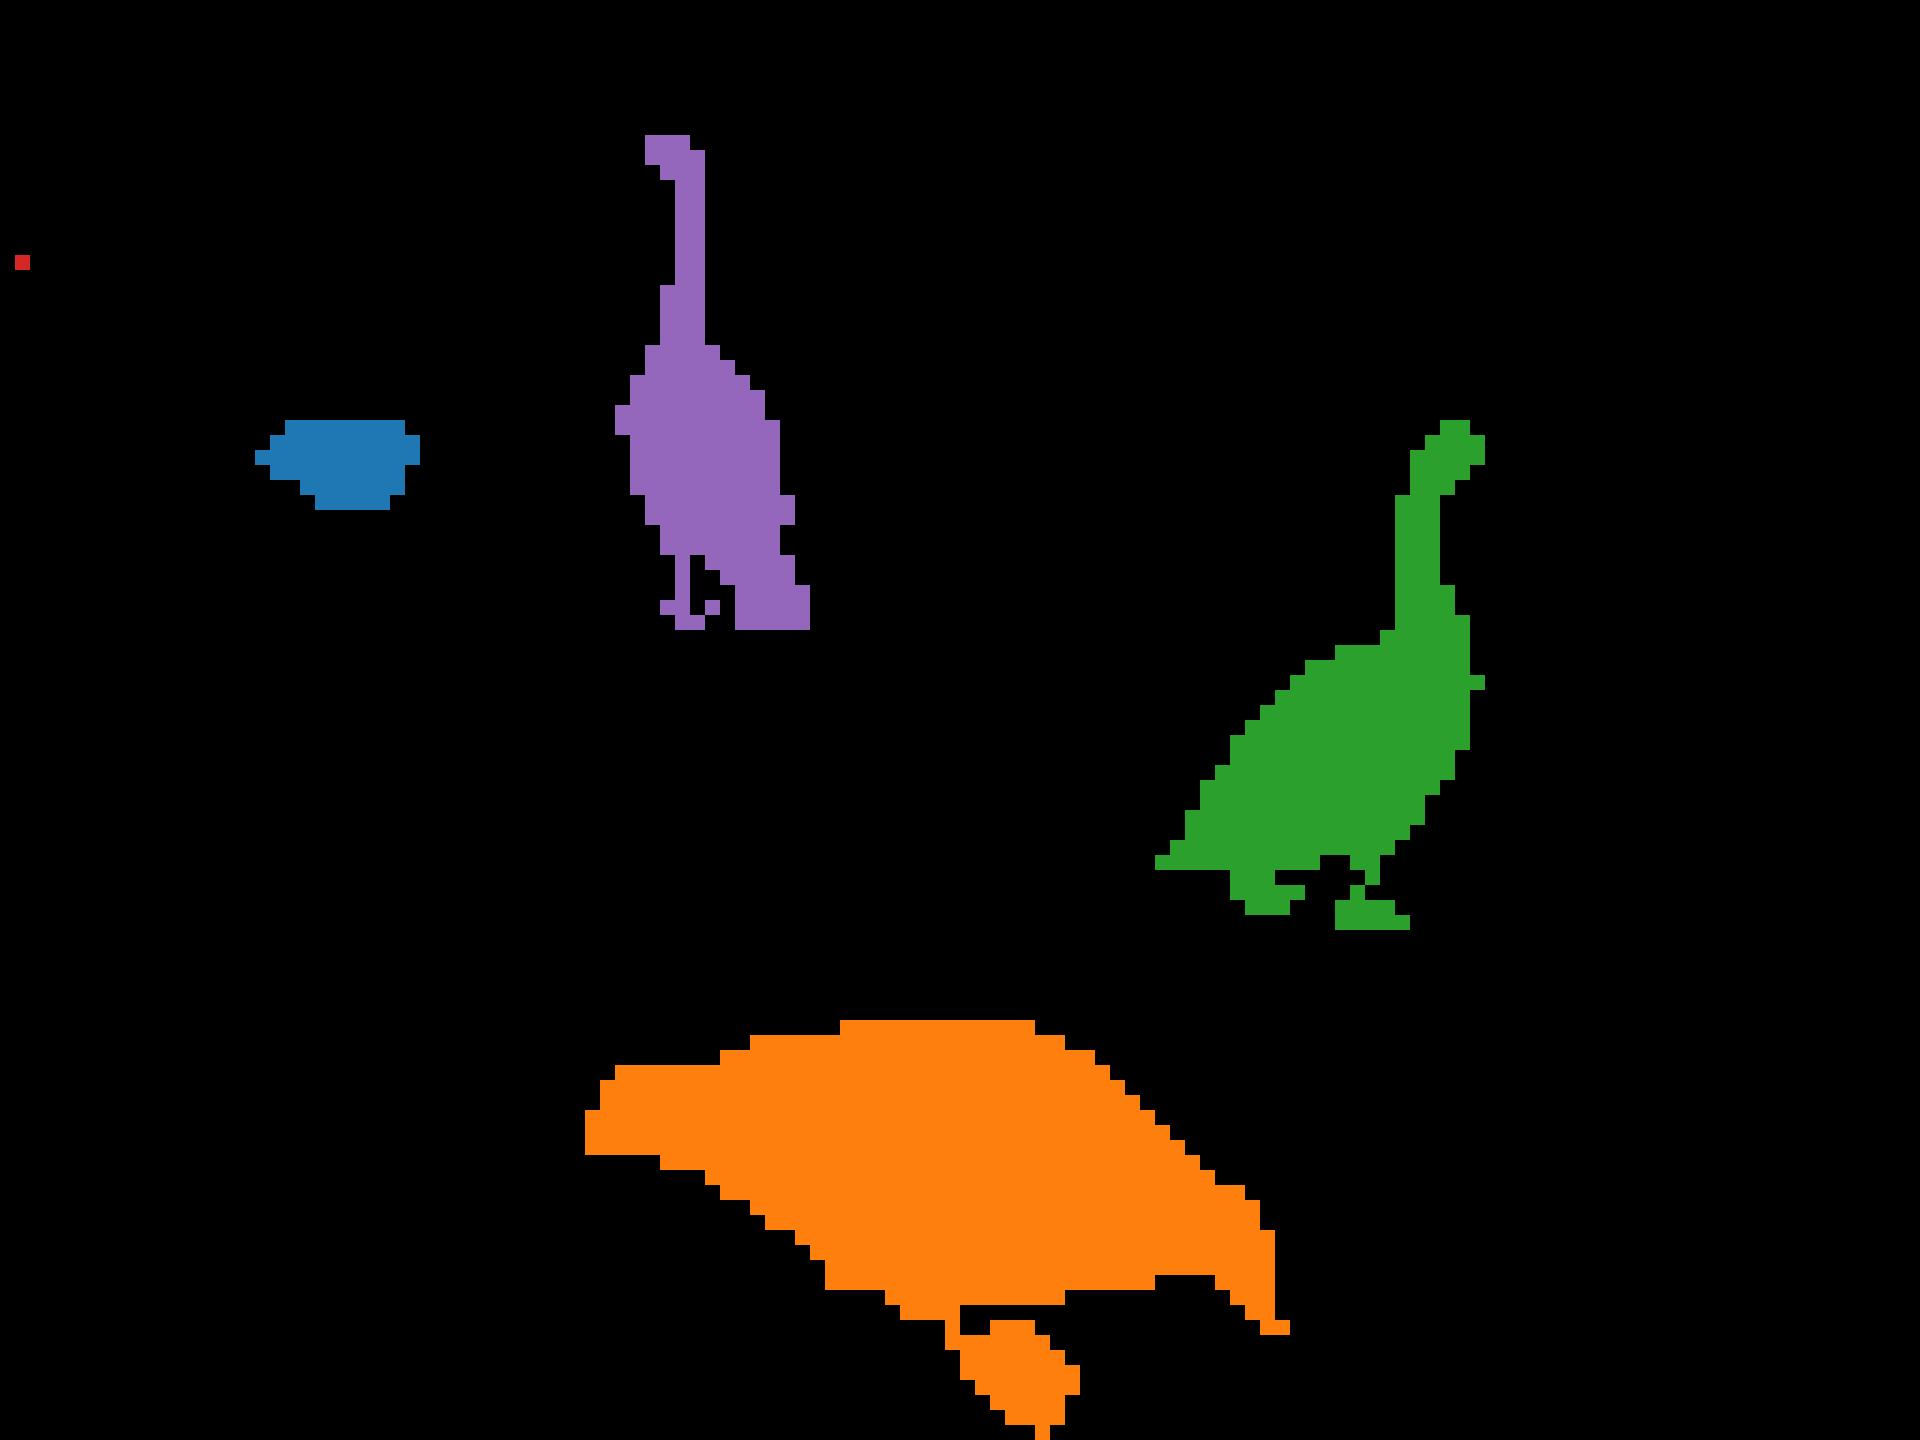
\includegraphics[width=\textwidth]{images/segmentation_tracking/ducks/all_obj/000121.jpg}
        \caption*{Frame 120}
    \end{subfigure}
    \caption{
        Segmentation tracking example.
        Given the ground-truth instance segmentation masks for the initial frame, we propagate the instance labels to subsequent frames according to patch similarity in the feature space of DINOv3.
        The input resolution is \(2048{\times}1536\) pixels, resulting in \(128{\times}96\) patches.
    }
    \label{fig:segmentation-tracking-example}
\end{figure}

\subsubsection{Video Classification}
\label{sec:results-video-classification}

The previous results have shown the low-level temporal consistency of DINOv3's representations, allowing to accurately track objects in time. 
Going beyond, we evaluate in this section the suitability of its dense features for high-level video classification.
Similar to the setup of V-JEPA 2~\citep{assran2025vjepa2}, we train an \emph{attentive probe}---a shallow 4-layer transformer-based classifier---on top of patch features extracted from each frame.
This enables reasoning over temporal and spatial dimensions as the features are extracted independently per frame.
During evaluation, we either take a single clip per video, or use test-time augmentation (TTA) by averaging the predictions of 3 spatial and 2 temporal crops per video.
See \cref{app:exp-details:video-classification} for experimental details.
We run this evaluation on three datasets: UCF101~\citep{soomro2012ucf101}, Something-Something V2~\citep{goyal2017something}, and Kinetics-400~\citep{kay2017kinetics}, and report top-1 accuracy.
As an additional baseline, we report the performance of V-JEPA v2, a state-of-the-art SSL model for video understanding.


\begin{table}[t]
    \centering
    \small
    \caption{
        Video classification evaluation using attentive probes.
        We report top-1 accuracy on UCF101, Something-Something V2 (SSv2), and Kinetics-400 (K400).
        For each model, we report performance for evaluating a single clip per video, or applying test-time augmentation (TTA) by averaging the predicted probabilities from multiple clips.
    }
    \label{tab:results-video-classification}
    \begin{tabular}{@{}ll cc cc cc@{}}
        \toprule
        & & \multicolumn{2}{c}{UCF101} & \multicolumn{2}{c}{SSv2} & \multicolumn{2}{c}{K400} \\
        \cmidrule(lr){3-4} \cmidrule(lr){5-6} \cmidrule(lr){7-8}
        Method & ViT & Single & TTA & Single & TTA & Single & TTA \\
        \midrule
        \multicolumn{2}{@{}l}{\resultsTableHeaderAgg} & & & & & & \\
        AM-RADIOv2.5  & g/14  & 92.8 & 92.5 & 69.1 & 70.0 & 84.8 & 85.2 \\
        PEspatial    & G/14  & 92.7 & 92.8 & 66.4 & 68.4 & 83.5 & 84.8 \\
        \midrule
        \multicolumn{2}{@{}l}{\resultsTableHeaderWeakly} & & & & & & \\
        SigLIP~2    & g/16  & 93.6 & \bf 94.2 & 68.8 & 70.2 & 86.9 & 87.7 \\
        PEcore    & G/14  & 93.1 & 93.3 & 69.0 & 70.4 & \bf 87.9 & \bf 88.8 \\
        \midrule
        \multicolumn{2}{@{}l}{\resultsTableHeaderSelf} & & & & & & \\
        DINOv2     & g/14  & 93.5 & 93.8 & 67.4 & 68.4 & 84.4 & 85.6 \\
        V-JEPA 2   & g/16  & \bf 94.0 & 93.8 & \bf 73.8 & \bf 75.4 & 83.3 & 84.3 \\
        Web-DINO   & 7B/14 & 93.9 & 94.1 & 67.3 & 68.1 & 86.8 & 87.2 \\
        \midrule
        DINOv3     & 7B/16 & 93.5 & 93.5 & 70.1 & 70.8 & 87.8 & 88.2 \\
        \bottomrule
    \end{tabular}
\end{table}

\paragraph[Results]{Results (\cref{tab:results-video-classification})}
In line with the conclusion of the previous experiment, we find that DINOv3 can be successfully used for extracting strong video features.
As this evaluation involves training several layers of self-attention, the differences between models are less visible.
However, DINOv3 lands in the same range as PEcore and SigLIP~2, and clearly outperforms other models (DINOv2, AM-RADIO) across datasets.
UCF101 and K400 are appearance-focused, where strong category-level understanding of objects gives most of the performance.
SSv2 on the other hand, requires better understanding of motion---the dedicated video model V-JEPA v2 shines on this dataset.
Interestingly, the gap between DINOv3 and the weakly-supervised models is slightly bigger on this dataset.
This again confirms the suitability of DINOv3 to video tasks.


\subsection{DINOv3 has Robust and Versatile Global Image Descriptors}
\label{sec:results-global-features}

In this section, we evaluate DINOv3's ability to capture global image statistics. 
To this end, we consider classic classification benchmarks using linear probes (\cref{sec:results-classification-linear}) and instance retrieval benchmarks (\cref{sec:results-instance-rec}).
Again, we compare to the strongest publicly available image encoders.
In addition to the models from the previous section, we evaluate the two weakly supervised models AIMv2~\citep{fini2024multimodal}, trained using joint auto-regressive pixel and text prediction, and the massive EVA-CLIP-18B~\citep{sun2024eva}.


\subsubsection{Image Classification with Linear Probing}
\label{sec:results-classification-linear}

We train a linear classifier on top of DINOv3's output CLS token to evaluate the model on classification benchmarks.
We consider the ImageNet1k~\citep{deng2009imagenet} dataset and its variants to evaluate out-of-distribution robustness, and a suite of datasets from different domains to understand DINOv3's ability to distinguish fine-grained classes.
See \cref{app:exp-details:classification} for evaluation details.

\paragraph[Domain Generalization from ImageNet]{Domain Generalization from ImageNet (\cref{tab:results-imagenet-classification}) }
In this experiment, we train on ImageNet-\emph{train}, use ImageNet-\emph{val} as a \emph{validation set} to select hyperparameters, and transfer the best found classifier to different test datasets: ImageNet-\textbf{V2}~\citep{recht2019imagenet} and \textbf{ReaL}~\citep{beyer2020imagenetreal} are alternative sets of images and labels for ImageNet, used to test overfitting on the ImageNet validation set; \textbf{R}endition~\citep{hendrycks2021many} and \textbf{S}ketch~\citep{wang2019learning} show stylized and artificial versions of the ImageNet classes; \textbf{A}dversarial~\citep{hendrycks2021natural} and \textbf{Obj}ectNet~\citep{barbu2019objectnet} contain deliberately-chosen difficult examples; \textbf{C}orruptions~\citep{hendrycks2019benchmarking} measures robustness to common image corruptions.
For reference, we also list linear probing results from \citet{dehghani2023scaling} for ViTs trained using supervised classification on the massive JFT dataset (3B--4B images).
Note that these results follow a slightly different evaluation protocol and are not directly comparable to our results.

DINOv3 significantly surpasses all previous self-supervised backbones, with gains of +10\% on ImageNet-R, +6\% on -Sketch, +13\% on ObjectNet over the previously strongest SSL model DINOv2.
We note that the strongest weakly-supervised models, SigLIP~2 and PE, are now better than the strongest supervised ones (ViT-22B) on hard OOD tasks like ImageNet-A and ObjectNet. 
DINOv3 reaches comparable results on ImageNet-R and -Sketch, and, on the hard tasks ImageNet-A and ObjectNet, is closely behind PE, while exceeding SigLIPv2.
On ImageNet, while validation scores are 0.7--0.9 points behind SigLIPv2 and PE, the performance on the ``cleaner'' test sets -V2 and -ReaL is virtually the same.
Notably, DINOv3 achieves the best robustness to corruptions (ImageNet-C).
All in all, \emph{this is the first time that a SSL model has reached comparable results to weakly- and supervised models on image classification}---a domain which used to be the strong point of (weakly-)supervised training approaches.
This is a remarkable result, given that models like ViT-22B, SigLIP~2, and PE are trained using massive human-annotated datasets.
In contrast, DINOv3 learns purely from images, which makes it feasible to further scale/improve the approach in the future. 


\begin{table}[t]
    \centering
    \small
    \caption{
        Classification accuracy of linear probes trained on ImageNet1k with frozen backbones. 
        Weakly- and self-supervised models are evaluated with image resolution adapted to 1024 patch tokens (\ie $448 \times 448$ for patch size 14, $512 \times 512$ for patch size 16).
        For reference, we also list results from \citet{dehghani2023scaling} using a different evaluation protocol (marked with $^\ast$).
    }
    \label{tab:results-imagenet-classification}
    \begin{tabular}{@{}ll c ccc c cc c ccc@{}}
        \toprule
        & && \multicolumn{3}{c}{ImageNet} && \multicolumn{2}{c}{Rendition} && \multicolumn{3}{c}{Hard} \\ 
        \cmidrule{4-6} \cmidrule{8-9} \cmidrule{11-13}
        Method  & ViT  && Val & V2 & ReaL && R & S && A & C $\downarrow$ & Obj. \\
        \midrule
        \multicolumn{2}{@{}l}{\resultsTableHeaderSuper} && & & && & && & & \\
        \citet{zhai2022scaling}$^\ast$ & G/14 && 89.0 & 81.3 & 90.6 && 91.7 & --- && 78.8 & --- & 69.6 \\
        \citet{chen2023pali}$^\ast$ & e/14 && 89.3 & 82.5 & 90.7 && 94.3 & --- && 81.6 & --- & 71.5 \\
        \citet{dehghani2023scaling}$^\ast$ & 22B/14 && 89.5 & 83.2 & 90.9 && 94.3 & --- && 83.8 & --- & 74.3 \\
        \midrule
        \multicolumn{2}{@{}l}{\resultsTableHeaderAgg} && & & && & && & & \\
        AM-RADIOv2.5 & g/14 && 88.0 & 80.2 & 90.3 && 83.8 & 67.1 && 81.3 & 27.1 & 68.4 \\
        \midrule
        \multicolumn{2}{@{}l}{\resultsTableHeaderWeakly} && & & && & && & & \\
        PEcore      & G/14 && \bf 89.3 & \bf 81.6 & 90.4 && \bf 92.2 & \bf 71.9 && \bf 89.0 & 22.7 & \bf 80.2 \\
        SigLIP~2     & g/16 && 89.1 & 81.6 & \bf 90.5 && \bf 92.2 & 71.8 && 84.6 & 30.0 & 78.6 \\
        AIMv2        & 3B/14 && 87.9 & 79.5 & 89.7 && 82.3 & 67.1 && 74.5 & 29.5 & 69.0 \\
        EVA-CLIP     & 18B/14 && 87.9 & 79.3 & 89.5 && 85.2 & 64.0 && 81.6 & 33.0 & 71.9 \\  
        \midrule
        \multicolumn{2}{@{}l}{\resultsTableHeaderSelf} && & & && & && & & \\
        Web-DINO   & 7B/14 && 85.9 & 77.1 & 88.6 && 75.6 & 64.0 && 71.6 & 31.2 & 69.7 \\
        Franca     & g/14   && 84.8 & 75.3 & 89.2 && 67.6 & 49.5 && 56.5 & 40.0 & 54.5 \\
        DINOv2     & g/14   && 87.3 & 79.5 & 89.9 && 81.1 & 65.4 && 81.7 & 24.1 & 66.4 \\
        \midrule
        DINOv3     & 7B/16  && 88.4 & 81.4 & 90.4 && 91.1 & 71.3 && 86.9 & \bf 19.6 & 79.0 \\ 
        \bottomrule
    \end{tabular}
\end{table}

\paragraph[Finegrained Classification]{Finegrained Classification (\cref{tab:results-classification-fine})}

\begin{table}[t]
    \begin{minipage}[b][][b]{.53\linewidth}
        \centering
        \small
        \caption{Finegrained classification benchmarks. 
        Fine-S averages over 12 datasets, see \cref{app:tab:results-classification-vtab} for full results.}
        \label{tab:results-classification-fine}
        \begin{tabular}{@{}l@{\hspace{6pt}}l@{\hspace{8pt}}c@{\hspace{6pt}}c@{\hspace{6pt}}c@{\hspace{6pt}}c@{}}
        \toprule
        Method & ViT & Fine-S & Places & iNat18 & iNat21 \\
        \midrule
        \multicolumn{2}{@{}l}{\resultsTableHeaderAgg} &&&& \\
        AM-RADIOv2.5 & g/14 & 93.9 & 70.2 & 79.0 & 83.7 \\
        \midrule
        \multicolumn{2}{@{}l}{\resultsTableHeaderWeakly} &&&& \\        
        SigLIP~2      & g/16 & 93.7 & 70.5 & 80.7 & 82.7 \\
        PEcore       & G/14 & \bf 94.5 & \bf 71.3 & \bf 86.6 & 87.0 \\
        AIMv2         & 3B/14 & 92.9 & 70.7 & 80.8 & 83.2 \\
        EVA CLIP      & 18B/14 & 92.9 & 71.1 & 80.7 & 83.5 \\
        \midrule
        \multicolumn{2}{@{}l}{\resultsTableHeaderSelf} &&&& \\
        Franca   & g/14  & 87.7 & 64.6 & 61.4 & 70.6 \\
        DINOv2   & g/14  & 92.6 & 68.2 & 80.7 & 86.1 \\
        Web-DINO & 7B/14 & 90.2 & 69.6 & 65.3 & 74.1 \\
        \midrule
        DINOv3   & 7B/16 & 93.0 & 70.0 & 85.6 & \bf 89.8 \\
        \bottomrule
    \end{tabular}
    \end{minipage}%
    \hfill
    \begin{minipage}[b][][b]{.44\linewidth}
        \centering
        \small
        \caption{
            Instance recognition benchmarks. 
            See \cref{app:tab:results-instance-retrieval} for additional metrics.
        }
        \label{tab:results-instance-recognition}
        \setlength{\tabcolsep}{4pt}
        \begin{tabular}{@{}cccc@{}}
        \toprule
        Oxford-H & Paris-H & Met (GAP) & AmsterTime \\  %
        \midrule
        \\
        47.5 & 85.7 & 30.5 & 23.1 \\  %
        \midrule
        \\       
        25.1 & 60.9 & 13.9 & 15.5 \\  %
        32.7 & 68.9 & 10.6 & 23.1 \\  %
        28.8 & 71.4 & 29.5 & 14.6 \\  %
        27.1 & 65.6 &  0.5 & 18.9 \\  %
        \midrule
        \\
        14.3 & 51.6 & 27.2 & 21.1 \\  %
        58.2 & 84.6 & 44.6 & 48.9 \\  %
        31.2 & 80.3 & 35.2 & 30.6 \\  %
        \midrule
        \bf 60.7 & \bf 87.1 & \bf 55.4 & \bf 56.5 \\  %
        \bottomrule
        \end{tabular}
    \end{minipage}
\end{table}


We also measure DINOv3's performance when training linear probes on several datasets for fine-grained classification.
In particular, we report the accuracy on 3 large datasets, namely Places205~\citep{zhou2014learning} for scene recognition, and iNaturalist 2018~\citep{van2018inaturalist} and iNaturalist 2021~\citep{van2021benchmarking}) for detailed plant and animal-species recognition, as well as the average over 12 smaller datasets covering scenes, objects, and textures (as in \citet{oquab2024dinov2}, here termed Fine-S).
See also \cref{app:tab:results-classification-vtab} for individual results on those datasets.

We find that, again, DINOv3 surpasses all previous SSL methods.
It also shows competitive results compared to the weakly-supervised methods, indicating its robustness and generalization capability across diverse finegrained classification tasks.
Notably, DINOv3 attains the highest accuracy on the difficult iNaturalist21 dataset at 89.8\%, outperforming even the best weakly-supervised model PEcore with 87.0\%.

\subsubsection{Instance Recognition}
\label{sec:results-instance-rec}

To evaluate the instance-level recognition capabilities of our model, we adopted a non-parametric retrieval approach. Here, database images are ranked by their cosine similarity to a given query image, using the output CLS token.
We benchmark performance across several datasets: the Oxford and Paris datasets for landmark recognition~\citep{radenovic2018revisiting}, the Met dataset featuring artworks from the Metropolitan Museum~\citep{ypsilantis2021met}, and AmsterTime, which consists of modern street view images matched to historical archival images of Amsterdam~\citep{yildiz2022amstertime}.
Retrieval effectiveness is quantified using mean average precision for Oxford, Paris, and AmsterTime, and global average precision for Met.
See \cref{app:exp-details:recognition} for more evaluation details.

\paragraph[Results]{Results (\cref{tab:results-instance-recognition,app:tab:results-instance-retrieval})}
Across all evaluated benchmarks, DINOv3 achieves the strongest performance by large margins, \eg improving over the second best model DINOv2 by +10.8 points on Met and +7.6 points on AmsterTime.
On this benchmark, weakly-supervised models are lagging far behind DINOv3, with the exception of AM-RADIO, which is distilled from DINOv2 features.
These findings highlight the robustness and versatility of DINOv3 for instance-level retrieval tasks, spanning both traditional landmark datasets and more challenging domains such as art and historical image retrieval.




\subsection{DINOv3 is a Foundation for Complex Computer Vision Systems}
\label{sec:results-system-level}

The previous two sections already provided solid signal for the quality of DINOv3 in both dense and global tasks. 
However, these results were obtained under ``model probing'' experimental protocols, using lightweight linear adapters or even non-parametric algorithms to assess the quality of features.
While such simple evaluations allowed to remove confounding factors from involved experimental protocols, they are not enough to evaluate the full potential of DINOv3 as a foundational component in a larger computer vision system.
Thus, in this section, we depart from the lightweight protocols, and instead train more involved downstream decoders and consider stronger, task-specific baselines.
In particular, we use DINOv3 as a basis for 
(1) object detection with Plain-DETR (\cref{sec:results-detection}), 
(2) semantic segmentation with Mask2Former (\cref{sec:results-segmentation}), 
(3) monocular depth estimation with Depth Anything (\cref{sec:results-depth-estimation}), 
and (4) 3D understanding with the Visual Geometry Grounded Transformer (\cref{sec:results-vggt}).
These tasks are only intended as explorations for what is possible with DINOv3.
Still, we find that building on DINOv3 unlocks competitive or even state-of-the-art results with little effort.

\subsubsection{Object Detection}
\label{sec:results-detection}
As a first task, we tackle the long-standing computer vision problem of object detection.
Given an image, the goal is to provide bounding boxes for all instances of objects of pre-defined categories.
This task requires both precise localization and good recognition, as boxes need to match the object boundaries and correspond to the correct category.
While performance on standard benchmarks like COCO~\citep{Lin2014cocodataset} is mostly saturated, we propose to tackle this task with a \emph{frozen} backbone, only training a small decoder on top.

\paragraph{Datasets and Metrics}
We evaluate DINOv3 on object detection capabilities with the COCO dataset~\citep{Lin2014cocodataset}, reporting results on the COCO-VAL2017 split.
Additionally, we evaluate out-of-distribution performance on the COCO-O evaluation dataset~\citep{mao2023cocoo}. 
This dataset contains the same classes but provides input images under six distribution shift settings.
For both datasets, we report mean Average Precision (mAP) with IoU thresholds in \([0.5:0.05:0.95]\).
For COCO-O, we additionally report the effective robustness (ER).
Since COCO is a small dataset, comprising only 118k training images, we leverage the larger Objects365 dataset~\citep{shao2019objects365} for pre-training the decoder, as is common practice.

\paragraph{Implementation}
We build upon the Plain-DETR~\citep{lin2023plaindetr}, but make the following modification:
We do not fuse the transformer encoder into the backbone, but keep it as a separate module, similar to the original DETR~\citep{carion2020detr}, which allows us to keep the DINOv3 backbone completely frozen during training and inference.
To the best of our knowledge, this makes it \emph{the first competitive detection model to use a frozen backbone}.
We train the Plain-DETR detector on Objects365 for 22 epochs at resolution 1536, then one epoch at resolution 2048, followed by 12 epochs on COCO at resolution 2048.
At inference time, we run at resolution 2048.
Optionally, we also apply test-time augmentation (TTA) by forwarding the image at multiple resolutions (from 1536 to 2880).
See \cref{app:exp-details:detection} for full experimental details.

\paragraph[Results]{Results (\cref{tab:results-object-detection})}
We compare our system with four models: 
EVA-02 with a Cascade detector~\citep{fang2024eva},
EVA-02 with Co-DETR~\citep{zong2023detrs},
InternImage-G with DINO~\citep{wang2022internimage},
and PEspatial with DETA~\citep{bolya2025perception}.
We find that our lightweight detector (100M parameters) trained on top of a frozen DINOv3 backbone manages to reach state-of-the-art performance.
For COCO-O, the gap is pronounced, showing that the detection model can effectively leverage the robustness of the DINOv3.
Interestingly, our model outperforms all previous models with much fewer trained parameters, with the smallest comparison point still using more than 300M trainable parameters.
We argue that achieving such strong performance without specializing the backbone is an enabler for various practical applications: A single backbone forward can provide features that support multiple tasks, reducing compute requirements.

\begin{table}[t]
    \centering
    \small
    \caption{
        Comparison with state-of-the-art systems on object detection.
        We train a detection adapter on top of a \emph{frozen} DINOv3 backbone.
        We show results on the validation set of the COCO and COCO-O datasets, and report the mAP across IoU thresholds, as well as the effective robustness (ER).
        Our detection system based on DINOv3 sets a new state of the art. 
        As the InternImage-G detection model has not been released, we were unable to reproduce their results or compute COCO-O scores.
    }
    \label{tab:results-object-detection}
    \begin{tabular}{@{}ll c ccc cc cc@{}}
    \toprule
    && & \multicolumn{3}{c}{Parameters} & \multicolumn{2}{c}{COCO} & \multicolumn{2}{c}{COCO-O} \\
    \cmidrule(lr){4-6} \cmidrule(lr){7-8} \cmidrule(lr){9-10}
    Model    & Detector & FT & Encoder & Decoder & Trainable & Simple & TTA &  mAP & ER \\
    \midrule
    EVA-02          & Cascade   & \orangefire & 300M    & ---   &  300M          & 64.1 & ---    & 63.6 & 34.7 \\
    InternImage-G   & DINO      & \orangefire & 6B      & ---   & 6B            & 65.1 & 65.3   & --- & --- \\
    EVA-02          & Co-DETR   & \orangefire & 300M    & ---   & 300M            & 65.4 & 65.9   & 63.7 & 34.3 \\
    PEspatial      & DETA      & \orangefire & 1.9B    & \phantom{0}50M & 2B    & 65.3 & 66.0   & 64.0 & 34.7 \\
    \midrule
    DINOv3          & Plain-DETR & \bluesnow  & \phantom{00}7B    & 100M & 100M & \textbf{65.6} & \textbf{66.1} & \textbf{66.4} &  \textbf{36.8} \\
    \bottomrule
\end{tabular}
\end{table}


\subsubsection{Semantic Segmentation}
\label{sec:results-segmentation}
Following the previous experiment, we now evaluate on semantic segmentation, another long-standing computer vision problem.
This task also requires strong, well localized representations, and expects a dense per-pixel prediction.
However, opposed to object detection, the model does not need to differentiate instances of the same object.
Similar to detection, we train a decoder on top of a \emph{frozen} DINOv3 model.

\paragraph{Datasets and Metrics}
We focus our evaluation on the ADE20k dataset~\citep{zhou2017scene}, which contains 150 semantic categories across 20k training images and 2k validation images.
We measure performance using the mean Intersection over Union (mIoU).
To train the segmentation model, we additionally use the COCO-Stuff \citep{caesar2018coco} and Hypersim \citep{roberts2021hypersim} datasets.
Those contain 164k images with 171 semantic categories, and 77k images with 40 categories respectively. 

\paragraph{Implementation}
To build a decoder that maps DINOv3 features to semantic categories, we combine ViT-Adapter \citep{chen2022vitadapter} and Mask2Former \citep{cheng2021mask2former}, similar to prior work~\citep{wang2022image,wang2022internimage,wang2023onepeace}.
However, in our case, the DINOv3 backbone remains frozen during training.
In order to avoid altering the backbone features, we further modify the original ViT-Adapter architecture by removing the injector component.
Compared to baselines, we also increase the embedding dimensions from $1024$ to $2048$, to support processing the $4096$-dimensional output of the DINOv3 backbone.
We start by pre-training the segmentation decoder on COCO-Stuff for $80$k iterations, followed by $10$k iterations on Hypersim \citep{roberts2021hypersim}.
Finally, we train for 20k iterations on the training split of ADE20k and report results on the validation split. 
All training is done at an input resolution of 896.
At inference time we consider two setups: single-scale, \ie we forward images at training resolution, or multi-scale, \ie we average predictions at multiple image ratios between \({\times}0.9\) and \(1.1\) the original training resolution.
We refer to \cref{app:exp-details:segmentation-system} for more experimental details.

\paragraph[Results]{Results (\cref{tab:results-for-ade20k})}
We compare our model's performance with several state-of-the-art baselines, including 
BEIT-3 \citep{wang2022image}, 
InternImage-H \citep{wang2022internimage} and 
ONE-PEACE \citep{wang2023onepeace}, and report results on additional datasets in \cref{app:tab:semantic-segmentation-other-datasets}.
Our segmentation model based on the frozen DINOv3 backbone reaches state-of-the-art performance, equaling that of ONE-PEACE ($63.0$ mIoU).
It also improves over all prior models on the COCO-Stuff~\citep{caesar2018coco} and VOC 2012~\citep{pascal-voc-2012} datasets.
As semantic segmentation requires accurate per-pixel predictions, vision transformer backbones pose a fundamental problem.
Indeed, the 16 pixel-wide input patches make the granularity of the prediction relatively coarse---encouraging solutions like ViT-Adapter. 
On the other hand, we have shown that we can obtain high-quality feature maps, even at very high resolutions up to 4096 (\cf \cref{fig:intro:dense-quality,fig:visualization-extreme-resolutions}); this corresponds to dense feature maps 512-tokens wide.
We hope that future work will be able to leverage these high-resolution features to reach state-of-the-art performance without having to rely on heavy decoders like ViT-Adapter with Mask2Former.


\begin{table}[t]
    \centering
    \small
    \caption{
        Comparison with state-of-the-art systems for semantic segmentation on ADE20k.
        We evaluate the model in a single- or multi-scale setup (respectively Simple and TTA).
        Following common practice, we run this evaluation at resolution 896 and report mIoU scores.
        BEIT3, ONE-PEACE and DINOv3 use a Mask2Former with ViT-Adapter architecture, and the decoder parameters take into account both.
        We report results on further datasets in \cref{app:tab:semantic-segmentation-other-datasets}
    }
    \begin{tabular}{lc ccc cc}
    \toprule
    & & \multicolumn{3}{c}{Parameters} &  \multicolumn{2}{c}{mIoU} \\
    \cmidrule(lr){3-5} \cmidrule(lr){6-7} 
    Model   &   FT       & Encoder & Decoder & Trainable &  Simple & TTA \\
    \midrule
    BEIT3           & \orangefire & 1.0B  & 550M & 1.6B &  62.0 & 62.8 \\  %
    InternImage-H   & \orangefire & 1.1B  & 230M & 1.3B &  62.5 & 62.9 \\  %
    ONE-PEACE       & \orangefire & 1.5B  & 710M & 2.2B &  62.0 & \textbf{63.0} \\  %
    \midrule
    DINOv3          & \bluesnow   & \phantom{0.}7B    & 927M & 927M &  \textbf{62.6} & \textbf{63.0} \\
    \bottomrule
    \end{tabular}
    \label{tab:results-for-ade20k}
\end{table}





\subsubsection{Monocular Depth Estimation}
\label{sec:results-depth-estimation}

We now consider building a system for monocular depth estimation.
To do so, we follow the setup of Depth Anything V2 (DAv2)~\citep{yang2024depthanythingv2}, a recent state-of-the-art method.
The key innovation of DAv2 is to use a large collection of synthetically generated images with ground truth depth annotations.
Critically, this relies on DINOv2 as a feature extractor that is able to bridge the \emph{sim-to-real} gap, a capability that other vision backbones like SAM~\citep{kirillov2023segment} do not show~\citep{yang2024depthanythingv2}.
Thus, we swap DINOv2 with DINOv3 in the DAv2 pipeline to see if we can achieve similar results.

\paragraph{Implementation}
Like DAv2, we use a Dense Prediction Transformer (DPT)~\citep{ranftl2021vision} to predict a pixelwise depth field, using features from four equally spaced layers of DINOv3 as input.
We train the model using the set of losses from DAv2 on DAv2's synthetic dataset, increasing the training resolution to $1024 \times 768$ to make use of DINOv3's high resolution capabilities.
In contrast to DAv2, we \emph{keep the backbone frozen} instead of finetuning it, testing the out-of-the-box capabilities of DINOv3.
We also found it beneficial to scale up the DPT head to obtain the full potential DINOv3 7B's larger features.
See \cref{app:exp-details:depth-system} for details.

\paragraph{Datasets and Metrics}
We evaluate our model on 5 real-world datasets (NYUv2~\citep{silberman2012indoor}, KITTI~\citep{geiger2013vision}, ETH3D~\citep{schoeps2017multiview}, ScanNet (from \citet{ke2025marigold}) and DIODE~\citep{vasiljevic2019diode}) in the zero-shot scale-invariant depth setup, similar to \citet{ranftl2020towards,ke2025marigold,yang2024depthanythingv2}.
We report the standard metrics absolute relative error (ARel) (lower is better) and $\delta_1$ (higher is better).
We refer to~\citet{yang2024depthanythingv1} for a description of those metrics.

\paragraph[Results]{Results (\cref{tab:results-depth-estimation-system-level})}
We compare to the state of the art for relative depth estimation: MiDaS~\citep{ranftl2020towards}, LeReS~\citep{yin2021learning}, Omnidata~\citep{eftekhar2021omnidata}, DPT~\citep{ranftl2021vision}, Marigold in the ensemble version~\citep{ke2025marigold} and DAv2.
Our depth estimation model reaches a new state-of-the-art on all datasets, only lacking behind in ARel on DIODE compared to DPT.
Remarkably, this is possible using a \emph{frozen backbone}, whereas all other baselines need to finetune the backbone for depth estimation.
In addition, this validates that DINOv3 inherits DINOv2's \emph{strong sim-to-real capabilities}, a desirable property that opens up the possibility for downstream tasks to use synthetically generated training data.

\begin{table}[t]
  \centering
  \small
  \caption{
    Comparison with state-of-the-art systems for relative monocular depth estimation.
    By combining DINOv3 with Depth Anything V2~\citep{yang2024depthanythingv2}, we obtain a SotA model for relative depth estimation.
  }
  \label{tab:results-depth-estimation-system-level}
  \setlength{\tabcolsep}{3.8pt}
  \begin{tabular}{@{}l c c cc c cc c cc c cc c cc@{}}
    \toprule
    & && \multicolumn{2}{c}{NYUv2} && \multicolumn{2}{c}{KITTI} && \multicolumn{2}{c}{ETH3D} && \multicolumn{2}{c}{ScanNet} && \multicolumn{2}{c}{DIODE}\\
    \cmidrule{4-5} \cmidrule{7-8} \cmidrule{10-11} \cmidrule{13-14} \cmidrule{16-17}
    Method & FT && ARel $\downarrow$ & $\delta_1 \uparrow$ && ARel $\downarrow$ & $\delta_1 \uparrow$ && ARel $\downarrow$ & $\delta_1 \uparrow$ && ARel $\downarrow$ & $\delta_1 \uparrow$ && ARel $\downarrow$ & $\delta_1 \uparrow$ \\
    \midrule
    MiDaS     & \orangefire && 11.1 & 88.5 && 23.6 & 63.0 && 18.4 & 75.2 && 12.1 & 84.6 && 33.2 & 71.5 \\
    LeReS     & \orangefire &&  9.0 & 91.6 && 14.9 & 78.4 && 17.1 & 77.7 &&  9.1 & 91.7 && 27.1 & 76.6 \\
    Omnidata  & \orangefire &&  7.4 & 94.5 && 14.9 & 83.5 && 16.6 & 77.8 &&  7.5 & 93.6 && 33.9 & 74.2 \\
    DPT       & \orangefire &&  9.8 & 90.3 && 10.0 & 90.1 &&  7.8 & 94.6 &&  8.2 & 93.4 && \textbf{18.2} & 75.8 \\
    Marigold  & \orangefire &&  5.5 & 96.4 &&  9.9 & 91.6 &&  6.5 & 96.0 &&  6.4 & 95.1 && 30.8 & 77.3 \\
    DAv2 (ViT-g) & \orangefire  &&  4.4 & 97.9 &&  7.5 & 94.7 && 13.1 & 86.5 && ---   & ---   && ---   & ---   \\
    \midrule
    DINOv3   & \bluesnow  &&  \textbf{4.3} & \textbf{98.0} &&  \textbf{7.3} & \textbf{96.7} &&  \textbf{5.4} & \textbf{97.5} &&  \textbf{4.4} & \textbf{98.1} && 25.6 & \textbf{82.2} \\
  \bottomrule
  \end{tabular}
\end{table}


\subsubsection{Visual Geometry Grounded Transformer with DINOv3}
\label{sec:results-vggt}

Finally, we consider 3D understanding with the recent Visual Geometry Grounded Transformer (VGGT)~\citep{wang2025vggt}.
Trained on a large set of 3D-annotated data, VGGT learns to estimate all important 3D attributes of a scene, such as camera intrinsics and extrinsics, point maps, or depth maps, in a single forward pass.
Using a simple, unified pipeline, it reaches state-of-the-art results on many 3D tasks while being more efficient than specialized methods---constituting a major advance in 3D understanding.

\paragraph{Implementation}
VGGT uses a DINOv2-pretrained backbone to obtain representations for different views of a scene, before fusing them with a transformer.
Here, we simply swap the DINOv2 backbone with DINOv3, using our ViT-L variant (see \cref{sec:family}) to match DINOv2 ViT-L/14 in the original work.
We run the same training pipeline as VGGT, including finetuning of the image backbone.
We switch the image resolution from $518 \times 518$ to $592 \times 592$ to accommodate DINOv3's patch size 16 and keep the the results comparable to VGGT. We additionally adopt a small number of hyperparameter changes detailed in \cref{app:exp-details:vggt}.

\begin{table}[t]
    \caption{
        3D understanding using Visual Geometry Grounded Transformer (VGGT)~\citep{wang2025vggt}. 
        Simply by swapping DINOv2 for DINOv3 ViT-L as the image feature extractor in the VGGT pipeline, we are able to obtain state-of-the-art results on various 3D geometry tasks.
        We reproduce baseline results from~\citet{wang2025vggt}. %
        We also report methods using ground truth camera information, marked with $^\ast$. 
        Camera pose estimation results are reported with AUC@30.  
    }
    \label{tab:results-vggt}
    \begin{subtable}{0.3\linewidth}
        \centering
        \small
        \caption{Camera pose estimation.}
        \label{tab:results-vggt-camera-pose}
        \setlength{\tabcolsep}{3pt}
        \begin{tabular}{@{}lcc@{}}
        \toprule
        Method & Re10K & CO3Dv2 \\
        \midrule
        DUSt3R & 67.7 & 76.7 \\
        MASt3R & 76.4 & 81.8 \\
        VG GSfM v2 & 78.9 & 83.4 \\
        CUT3R & 75.3 & 82.8 \\
        FLARE & 78.8 & 83.3 \\
        VGGT & 85.3 & 88.2 \\
        \midrule
        DINOv3 & \bf 86.3 & \bf 89.6 \\
        \bottomrule
        \end{tabular}
    \end{subtable}%
    \hfill
    \begin{subtable}{0.35\linewidth}
        \centering
        \caption{Multi-view estimation on DTU.}
        \label{tab:results-vggt-mvs}
        \setlength{\tabcolsep}{2pt}
        \small
        \begin{tabular}{@{}lccc@{}}
        \toprule
        Method & Acc.$\downarrow$ & Comp.$\downarrow$ & Overall$\downarrow$ \\
        \midrule
        \textcolor{gray}{Gipuma$^\ast$} & \textcolor{gray}{0.283} & \textcolor{gray}{0.873} & \textcolor{gray}{0.578} \\
        \textcolor{gray}{CIDER$^\ast$} & \textcolor{gray}{0.417} & \textcolor{gray}{0.437} & \textcolor{gray}{0.427} \\
        \textcolor{gray}{MASt3R$^\ast$} & \textcolor{gray}{0.403} & \textcolor{gray}{0.344} & \textcolor{gray}{0.374} \\
        \textcolor{gray}{GeoMVSNet$^\ast$} & \textcolor{gray}{0.331} & \textcolor{gray}{0.259} & \textcolor{gray}{0.295} \\
        DUSt3R & 2.677 & 0.805 & 1.741 \\
        VGGT & 0.389 & 0.374 & 0.382 \\
        \midrule
        DINOv3  & \bf 0.375 & \bf 0.361 & \bf 0.368 \\
        \bottomrule
        \end{tabular}
    \end{subtable}%
    \hfill
    \begin{subtable}{0.315\linewidth}
        \centering
        \small
        \caption{View matching on ScanNet-1500.}
        \label{tab:results-vggt-view-matching}
        \setlength{\tabcolsep}{3pt}
        \begin{tabular}{@{}lcc@{}}
        \toprule
        Method & AUC@5 & AUC@10 \\
        \midrule
        SuperGlue & 16.2 & 33.8 \\
        LoFTR & 22.1 & 40.8 \\
        DKM & 29.4 & 50.7 \\
        CasMTR & 27.1 & 47.0 \\
        Roma & 31.8 & 53.4 \\
        VGGT & 33.9 & 55.2 \\
        \midrule
        DINOv3 & \bf 35.2 & \bf 56.1 \\
        \bottomrule
        \end{tabular}
    \end{subtable}
\end{table}

\paragraph{Datasets and Metrics}
Following \citet{wang2025vggt}, we evaluate on camera pose estimation on the Re10K~\citep{zhou2018stereo} and CO3Dv2~\citep{reizenstein2021common} datasets, dense multi-view estimation on DTU~\citep{jensen2014large}, and two-view matching on ScanNet-1500~\citep{dai2017scannet}.
For camera pose estimation and two-view matching, we report the standard area-under-curve (AUC) metric.  %
For multi-view estimation, we report the smallest L2-distance between prediction to ground truth as ``Accuracy'', the smallest L2-distance from ground truth to prediction as ``Completeness'' and their average as `Overall''.
We refer to \citet{wang2025vggt} for details about method and evaluation.

\paragraph[Results]{Results (\cref{tab:results-vggt})}
We find that VGGT equipped with DINOv3 \emph{further improves over the previous state-of-the-art} set by VGGT on all three considered tasks---using DINOv3 leads to clear and consistent gains.
This is encouraging, given that we only applied minimal tuning for DINOv3.
These tasks span different levels of visual understanding: high-level abstraction of scene content (camera pose estimation), dense geometric prediction (multi-view depth estimation), and fine-grained pixel-level correspondence (view matching).
Together with the previous results on correspondence estimation (\cref{sec:results-correspondence-estimation}) and depth estimation (\cref{sec:results-depth-estimation}), we take this as further empirical evidence for the strong suitability of DINOv3 as a basis for 3D tasks.
Additionally, we anticipate further improvements from using the larger DINOv3 7B model. 
